%#############################################################
% Autor: Prof. Dr. Kai Luppa
% Fachhochschule Dortmund Fachbereich Informations- und Elektrotechnik
% Stand: Version2.0, 16.11.2017
%
% Dies ist eine Vorlage für Abschlussarbeiten (Bachelor Thesis, Betriebliche Praxis, 
% Projektarbeiten, etc.) Der Dokumentenaufbau (Titelblatt sowie Reihenfolge
% der Verzeichnisse und Anhänge) sollte nicht verändert werden.
%
% In der Päambel sind ggf. BibTex-Datei und die verwendeten Abkürzungen
% anzupassen (beides direkt vor \begin{document}). Im Dokument werden
% Formatierungsvorlagen angewendet, die so als Grundlage von Abschlussarbeiten 
% im Labor für Energieautomatisierung verwendet werden sollten. 
%
% Das Prozentzeichen bedeutet übrigens den Beginn eines Kommentars ;-)
%
% Zum Übersetzen in das PDF-Format die folgenden Aufrufe starten: 
% pdflatex _LaTeX_Vorlage_FHDO_V2.tex
% bibtex _LaTeX_Vorlage_FHDO_V2
% pdflatex _LaTeX_Vorlage_FHDO_V2.tex
% pdflatex _LaTeX_Vorlage_FHDO_V2.tex


%#############################################################
% Hier beginnt die Präambel
\documentclass[a4paper,11pt,ngerman,headsepline,bibtotoc,liststotoc,numbers=noenddot]{scrreprt}
 
\usepackage[T1]{fontenc}
\usepackage[utf8]{inputenc}
\usepackage[ngerman]{babel}
\usepackage{footmisc} % für Fußnotenreferenzen mit \footref{}
\usepackage[printonlyused]{acronym} % für das Abkürzungsverzeichnis
\usepackage{graphicx} % für die Abbildungen
\usepackage{float} % für die Gleitumgebung (Abbildungen, Tabellen, Listings)
\usepackage{listings} % für die Listings
\usepackage{color} % für grauen Hintergrund der Listings
\usepackage[sorting=nty,backend=bibtex8]{biblatex} % für das Literaturverzeichnis
\usepackage[colorlinks=false]{hyperref} % PDF-Inhaltsverzeichnis und Links einschalten, wird nicht gedruckt
\usepackage{array} % für die zentrierten Spalten mit vorgegebener Breite in einer Tabelle (longtable)
\usepackage[acronym,nomain,nonumberlist,toc]{glossaries} % für die Abkürzungsliste
\usepackage{pdfpages} % zum Einbinden von PDF-Dokumenten
\usepackage{chngcntr} % für durchgängige Fussnotenzählung
\usepackage{codestyle}

\usepackage{xcolor}
\usepackage[left=2.5cm, right=2.5cm, top=2.5cm, bottom=2.5cm]{geometry}

\counterwithout{footnote}{chapter} % durchgängige Fussnotenzählung

\DefineBibliographyStrings{ngerman}{bibliography = {Literaturverzeichnis}} % Titel für Literatur ändern


\definecolor{grey}{rgb}{0.95,0.95,0.95} % definiere grau für Hintergrund der Listings
\definecolor{blau}{rgb}{0,0.8,1.0} % definiere blau für Füllfarbe
\definecolor{grua}{rgb}{0.7529,0.7529,0.7529} % definiere grau für Füllfarbe
\definecolor{gelb}{rgb}{1.0,1.0,0} % definiere gelb für Füllfarbe
\definecolor{gren}{rgb}{0,0.5,0} % definiere grün für Füllfarbe
\definecolor{rot}{rgb}{1.0,0,0} % definiere blau für Füllfarbe
\definecolor{hellgren}{rgb}{0.251,1,0.255} % definiere blau für Füllfarbe
\definecolor{dunkelgren}{rgb}{0,0.25,0} % definiere blau für Füllfarbe
\definecolor{grua2}{rgb}{0.5,0.5,0.5} % definiere blau für Füllfarbe
% Einstellungen für Listings
%\lstset{captionpos=b, 
%	language=java, 
%	alsolanguage=php,
%	alsolanguage=c,
%	numbers=left,
%	breaklines=true,
%	tabsize=3, 
%	basicstyle=\ttfamily\small,
%	backgroundcolor=\color{grey},
%	numberstyle=\scriptsize, 
%	frame=single, 
%	framerule=0.1pt,
%	showstringspaces=false,
%}

\setcounter{secnumdepth}{3} % drei Abschnitts-Gliederungstiefen
\setcounter{tocdepth}{3} % drei Abschnittsgliederungstiefen im Inhaltsverzeichnis anzeigen

\setlength{\parindent}{0mm} % Länge des Einzungs beim Absatz -> 0mm: kein Einzug
\setlength{\parskip}{0cm} % Vertikale Abstand zu einem neuen Absatz

\renewcommand{\lstlistlistingname}{Quelltextverzeichnis}% Änderung von Listings nach Quelltextverzeichnis
\renewcommand{\lstlistingname}{Quelltext} % Änderung von Listing nach Quelltext
\renewcommand{\arraystretch}{1.2} % Tabellenzeilenabstand um Faktor 1.2 vergrößern
\newcolumntype{C}[1]{>{\centering\arraybackslash}p{#1}} % zentrierte Spalten mit Breitenangabe 
\newcolumntype{R}[1]{>{\raggedleft\arraybackslash}p{#1}} % rechtsbündig mit Breitenangabe 
\newcolumntype{L}[1]{>{\raggedright\arraybackslash}p{#1}} % linksbündig mit Breitenangabe 
\renewcommand*{\glspostdescription}{} % Den Punkt am Ende jeder Beschreibung deaktivieren

\newcommand{\afzsm}[1]{\dq #1\dq}
\newcommand{\afzde}[1]{\glqq #1\grqq}
\newcommand{\afzfr}[1]{\flqq #1\frqq}

\sloppy % Immer im Blocksatz bleiben

\makeglossaries % erstelle die Glossaries, hier nur das Abkürzungsverzeichnis


%**********************************************************************************
% In der Präamble sind nur die folgenden zwei Punkte 
% 1. ggf. BibTex-Datei
% 2. Verwendete Abkürzungen 
% anzupassen

%----------------------------------------------------------------------
% Hier ggf. die BibTex-Datei anpassen (wenn anderer Dateiname gewählt wurde) 

\bibliography{Literatur} % verwende die Datei Literatur.bib im selben Verzeichnis

%----------------------------------------------------------------------
% Hier die Abkürzungsliste bearbeiten 
\newacronym{ac:tcpip}{TCP/IP}{Transmission Control Protocol / Internet Protocol}
%\newacronym{ac:ew}{EW}{Energiewirtschaft}
%\newacronym{ac:ew30}{EW30}{Energieautomation}
%\newacronym{ac:fb}{FB}{Fachbereich}
%\newacronym{ac:fhdo}{FHDO}{Fachhochschule Dortmund}
%\newacronym{ac:il}{IL}{Energieinformationstechnik und Leitsysteme}
%\newacronym{xyz}{XYZ}{lXXX YYY ZZZ}
\newacronym{ac:gpio}{GPIO}{General-Purpose Input/Output}
\newacronym{ac:gui}{GUI}{Graphical User Interface}
\newacronym{ac:JSON}{JSON}{JavaScript Object Notation}
\newacronym{ac:LED}{LED}{Light Emitting Diode}
\newacronym{ac:LCD}{LCD}{Liquid Crystal Display}
\newacronym{ac:ip}{IP}{Internetprotocol}
\newacronym{ac:tia}{TIA}{Totally Integrated Automation}
\newacronym{ac:pet}{PET}{Polyethylenterephthalat}
\newacronym{ac:sps}{SPS}{Speicherprogrammierbare Steuerung}
\newacronym{ac:fu}{FU}{Frequenzumrichter}


\newcommand{\ptitel}{\emph{Mein Projekt-Titel}}
\newcommand{\paufgabe}{\emph{Entwicklung einer hyperdüper Netzleittechnik für die Netze von Übermorgen}}
\newcommand{\absatz}{\\[0.2cm]}
%---------------------------------------------------------------------
% Hier Definition von eingegebenen Quellcode
 \definecolor{darkgreen}{rgb}{0.0, 0.42, 0.24}
 \definecolor{blue-violet}{rgb}{0.55, 0.0, 0.55}
%\lstset{
%	language=python, 				% Setzt die Sprache
%	basicstyle=\scriptsize\ttfamily, 	% Setzt den Standardstil
%	keywordstyle=\color{blue-violet}\bfseries,	% Setzt den Stil für Schlüsselwörter
%	identifierstyle=\color{blue},		% Identifier bekommen keine gesonderte formatierung
%	commentstyle=\color{darkgreen},		% Stil für Kommentare
%	stringstyle=\ttfamily, 			% Stil für Strings (gekennzeichnet mit "String")
%	breaklines=true, 			% Zeilen werden umgebrochen
%	numbers=left, 				% Zeilennummern links
%	numberstyle=\tiny, 			% Stil für die Seitennummern
%	frame=single, 				% Rahmen
%	backgroundcolor=\color{white}, 	% Hintergrundfarbe
%	caption={Python-Code}, 			% Caption
%	tabsize=4				% Größe der Tabulatoren
%}

%#############################################################
% Hier beginnt das Dokument
\begin{document}

%----------------------------------------------------------------------
% Titelseite
\begin{titlepage}
	\titlehead{\flushleft
\includegraphics[width=1.0\linewidth]{./_bilder/__fhdologo.png}}%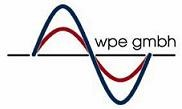
\includegraphics[width=3.64cm,height=2.18cm]{./_bilder/wpe.png}}

\subject{
	Betriebliche Praxis
} 
\title{
	Bericht über die Erstellung der Benutzeroberfläche der SIEMENS Comfort Pannels im SIEMENS TIA-Portal
}
\author{	
	%Aron von dem Berge\\ 
	%\small{Matrikelnummer 7201810}\\
	Frederik Rath\\ 
	\small{Matrikelnummer 7202624}\\
	%Lorena Sträßer\\ % hier den Namen anpassen
	%\small{Matrikelnummer 7201327} \\% hier die Matrikelnummer anpassen
} 
\date{\today} % das aktuelle Erstellungsdatum
\publishers{
	\begin{tabular}{ll}
		Erstprüfer: & Prof. Dr.-Ing. Nick Raabe \\ 
		Zweitprüfer: &   Dipl.-Ing. Guido Grzeskowiak  \\
	\end{tabular} 
}
\maketitle % erstelle Titelseite
\thispagestyle{empty} % ohne Seitennummerierung
\end{titlepage}


%----------------------------------------------------------------------
% Optional: Vorwort oder Danksagung, ggf. diesen Block löschen
%\newpage
%\chapter*{Vorwort / Hinweise / Danksagung}
%Text ...
%\thispagestyle{empty} % ohne Seitennummerierung

%----------------------------------------------------------------------
% Eidesstattliche Erklärung, bei Betrieblicher Praxis etc. diesen Block löschen
% WICHTIG: Prüfen, ob u. g. Text aktuell ist
%\newpage
%\chapter*{Erklärung}
%„Hiermit versichere ich an Eides statt, dass ich die vorliegende Arbeit %selbständig
%und ohne die Benutzung anderer als der angegebenen Hilfsmittel angefertigt
%habe. Alle Stellen, die wörtlich oder sinngemäß aus veröffentlichten und nicht
%veröffentlichten Schriften entnommen wurden, sind als solche kenntlich gemacht.“
%\\
%\vspace*{3cm}\\
%Dortmund, \the\day.\the\month.\the\year \hspace*{3cm} \rule{8cm}{0.75pt} \\ 
%\hspace*{6,5cm} Unterschrift, Lorena Sträßer
%\vspace*{3cm}\\
%Dortmund, \the\day.\the\month.\the\year \hspace*{3cm} \rule{8cm}{0.75pt} \\ 
%\hspace*{6,5cm} Unterschrift, Aron von dem Berge
%\vspace*{3cm}\\
%Dortmund, \the\day.\the\month.\the\year \hspace*{3cm} \rule{8cm}{0.75pt} \\ 
%\hspace*{6,5cm} Unterschrift, Frederik Rath
%\thispagestyle{empty}

%----------------------------------------------------------------------
% Abstract, bei Betrieblicher Praxis etc. diesen Block löschen
%\newpage
%\chapter*{Abstract}
%Hier eine halbe Seite inhaltliche Zusammenfassung der Arbeit in englischer Sprache ...
%\\[1cm]
%Hier eine halbe Seite inhaltliche Zusammenfassung der Arbeit in deutscher Sprache ...
%\thispagestyle{empty}

%\newpage

%----------------------------------------------------------------------
% Verzeichnisse: Inhalt, Abbildungen, ggf. Tabellen, ggf. Listings, Abkürzungen
% alle Seiten der Verzeichnisse werden in römischen Zahlen nummeriert
\setcounter{page}{1} % ab hier mit Seite 1 beginnen
\pagenumbering{Roman} % römische Nummerierung einschalten
\tableofcontents % erstelle Inhaltsangabe
%\newpage
%\listoffigures % erstelle Abbildungsverzeichnis
%\newpage
%\listoftables % erstelle Tabellenverzeichnis
%\newpage
%\lstlistoflistings % erstelle Listing-Verzeichnis
\newpage
\glossarystyle{long} % Formatstil für das Abkürzungsverzeichnis
\printglossary[title={Abkürzungen},toctitle={Abkürzungen}] % erstelle Abkürzungsverzeichnis
%\clearpage
\newpage

%----------------------------------------------------------------------
% Ab hier beginnt der Text, es werden noch folgende Einstellungen vorgenommen:
\pagenumbering{arabic} % arabische Nummerierung einschalten 
\setcounter{page}{1} % ab hier mit Seite 1 beginnen
\pagestyle{headings} % Kapitelüberschrift in den Seitenkopf übernehmen

%**********************************************************************************
\chapter*{Einleitung}
%1-1,5 Seiten\\[0,2cm]
%In 3 Teile Gliedern:\\ [0,2cm]
%1. Motivation (nicht persönlich)\\
%2. Das technische Umfeld (Verwendung in der Steuerungstechnik, Smart Home, Fernsteuerung)\\
%3. Gliederung und Aufbau der Arbeit\\
%Motivation: Programmiersprache lernen, hardwarenah programmieren, Der Koffer, \\ Motivation zuhause mit dem licht an aus machen ob es nicht interessant wäre es von fern ein und aus zuschalten weg vom Koffer, grosse bürogebäude licht ausmachen können gleichzeitig überwachung stromverbrauch  \\

In dem folgenden Bericht zu der betrieblichen Praxis, welche bei der Firma WPE GmbH in Lünen durchgeführt wurde, geht es um die Erstellung einer Benutzeroberfläche eines SIEMENS Comfort Pannels mit Hilfe des \gls{ac:tia}-Portals. \\
Der Kunde hat für die Ansteuerung einer Mischer- und Abfüllanlage einen neuen Steuerschrank sowie einen Leistungsschrank in Auftrag gegeben. Dabei werden die vorhandenen Bedienelemente demontiert und durch einen im neuen Steuerschrank verbautes Touchpanel ersetzt, zudem wird der vorhandene Leistungsschrank angepasst und erweitert. Zusätzlich wird eine dezentrale Bedienstelle mit einem weiteren Touchpanel in einem Hängeschrank angebracht. Für die Motorsteuerung der einzelnen Förderschnecken werden Leitungsschutzschalter, Motorschutzschalter, Leistungsschütze und gegebenenfalls Frequenzumrichter im Leistungsschrank montiert.\\ 
Bei der Anlage handelt es sich um ein Greenfieldprojekt, bei dem die komplette Anlage von Grund auf entworfen, gezeichnet, geplant und aufgebaut wird. Den Entwurf der Anlage hat die Firma Günter Anlagenbau übernommen und die erforderlichen technischen Zeichnungen erstellt. Im weiteren Schritt werden die Schaltpläne für die Verdrahtung, die Kabeldimensionierung und die Erstellung der Programmierung von der Firma WPE durchgeführt.\\
Diese Sortier- und Mischeranlage besteht aus fünf Materialsilos, in die locker geliefertes Material aus LKWs geladen und gelagert wird, zwei BIG-BAG-Stationen, in die aus BIG-BAGs angeliefertes Material in das Verfahren eingeführt werden kann, drei Sortierern, 38 Material transportierende Förderschnecken und fünf Materialmischern. Das Ziel dieser Anlage ist aus geschredderten Einwegflaschen eine sortierte Mischung an Flakes zu erzeugen, die in die Mischer kommt und dort vermengt werden. Im nächsten Prozessschritt werden die vermischten Flakes in den Extruder weitergeleitet und zu neuem Plastikgranulat eingeschmolzen. Um die Farbe des Granulats zu steuern, sortieren die drei Sorter nach unterschiedlichen Prinzipen die Flakes aus. Der Sorter der Marke Tomra besitzt eine Kameratechnik, die in kürzester Zeit die einzelnen Bestandteile erkennen und nach Materialfarbe sortieren und Fremdkörper entfernen kann. Die zwei Unisorter sortieren mit Hilfe eines nahinfrarot Sortiersystems alle hellen Polymerarten und trennen diese  voneinander, dabei werden alle dunklen Störstoffe aussortiert. Durch die Förderschnecken können die Sorter gezielt mit Material versorgt werden und so die Farbtöne des gemischten Flakes für jeden der vier Mischern individuell gesteuert werden. Der fünfte Mischer kann als Überlauf verwendet werden, damit die letzten beiden Schnecken nicht voll laufen, falls der Mischer vorher kein Material aus der Förderschnecke bekommt. Der Mischer kann aber auch individuell befüllt werden, sodass es maximal fünf verschiedene Mischungen geben kann.\\
Diese Art der Wiederaufbereitung von Einwegflaschen kann einen enormen Beitrag dazu beitragen, dass der Verbrauch von Rohöl zur Plastikherstellung sinkt. Gerade in der heutigen Zeit, wo der Umweltschutz und Vermeidung von klimaschädlichen Treibhausgasen verringert und eingeschränkt werden soll. Ein großer Discounter verwendet für die neuen Einwegflaschen aus deren Eigenmarkensortiment nur noch Plastikgranulat aus recycelten \gls{ac:pet}-Flaschen. Zudem ist das Granulat sehr begehrt für die Herstellung von anderen Plastikprodukten. \\
Diese Dokumentation befasst sich mit der Planung und der Realisierung des Projektes. Es beginnt mit der Aufgabenstellung. Zu Beginn soll die Analyse der Planungsunterlagen bestehend aus Ein- und Ausgangslisten und Plänen durchgeführt werden. Danach soll eine Topologie der vernetzten \gls{ac:sps}-Komponenten erstellt werden, damit die \gls{ac:ip}-Adressen fest zugewiesen werden können. Abschließend soll eine Visualisierung für die Comfortpannels angefertigt werden, damit die Bedienung über beide Comfortpannels möglich ist.

Ich bins Tim
%---------------------------------------------------------------------
\chapter{Aufgabenstellung}

In diesem Kapitel wird die Aufgabenstellung beschrieben und die Ziele des Projektes definiert. 

\section{Analyse der Unterlagen}

Als erstes Ziel gilt es die vorliegenden Unterlagen durchzuarbeiten und zu analysieren. Dabei muss für jedes Betriebsmittel die Anzahl der Ein- und Ausgänge ermittelt werden und diese in die Ein- und Ausgangs Liste dokumentiert werden. Wenn dies abgeschlossen ist müssen mit der Anzahl aller Ein- und Ausgänge die digitalen und analogen Ein- und Ausgangskarten bestellt werden. Als nächstes müssen die Kabelquerschnitte der Zuleitungen für die Motoren berechnet werden. Dies geschieht anhand der Leitungslänge und des Nennstroms im Nennbetrieb, der aus den Leistungen in Abbildung \ref{fig:übersicht} berechnet werden kann. 

\begin{figure}[H] % H: figure wird an dieser Stelle eingefügt
	\centering{ % der Inhalt von figure wird zentriert ausgerichtet
		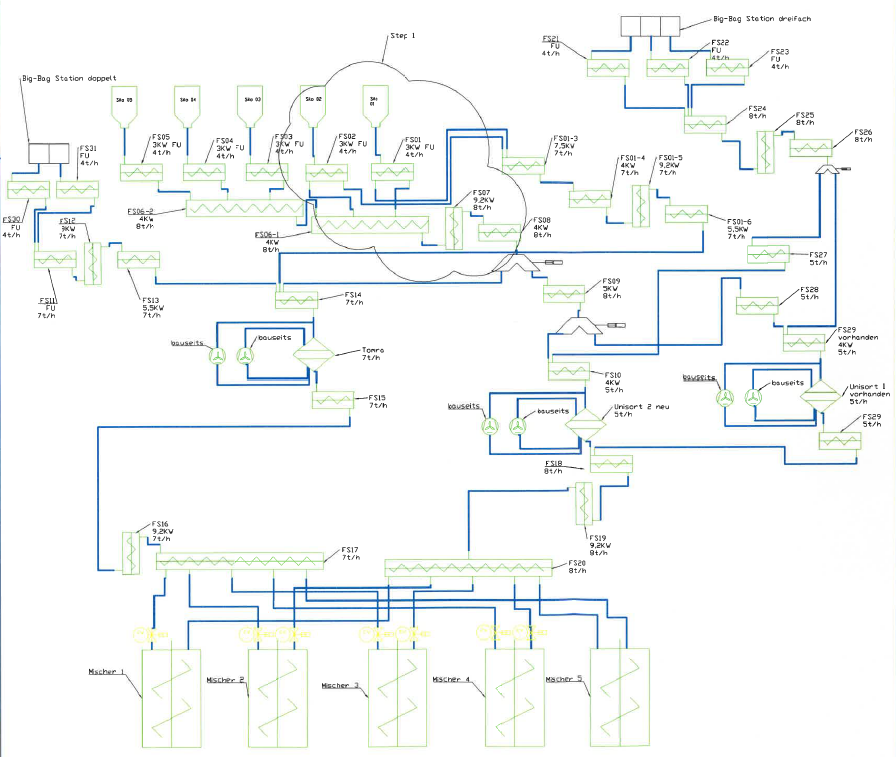
\includegraphics[width=14.85cm,height=10.5cm]{./_bilder/PID_Flakes.png} % 80-Prozent der Textbreite, nur PDF und PNG
		\caption[Übersicht der Antriebe]
		{Übersicht der Antriebe}
		% [...] ist für das Abbildungsverzeichnis ohne Fußnote, {...} Beschriftung mit Fußnote (\footnotetext{...})
		\label{fig:übersicht}
	} % schliesst \centering
\end{figure} % schliesst die Umgebung 


\section{Grafische Oberfläche}

Nachdem die Analyse der Unterlagen abgeschlossen ist, soll eine grafische Oberfläche im \gls{ac:tia}-Portal erzeugt werden. Mit der grafischen Oberfläche sollen alle Motoren gesteuert werden können. Dies bedeutet, dass die Motoren mit Direktantrieb ein- und ausgeschaltet und die Motoren mit einem \gls{ac:fu} in der Drehzahl verändert werden können. Ebenso sollen die Statusmeldungen der Motoren hinzugefügt werden, die zeigen, in welchem Zustand der Motor befindet. Ab hier wird die Steuerung in Gesamtübersicht, Silos, Big-Bag Stationen, Sorter und Mischer unterschieden. Durch das Tippen auf einzelne Motoren sollen Pop-Up Fenster erscheinen. In diesen Fenstern sollen Informationen zu dem Motor stehen, sich die Bedienung befinden, Störmeldungen angezeigt werden und weitere notwendige Schaltflächen. In der Gesamtübersicht soll keine Bedienung möglich sein. Dies ist nur in den vier anderen Ansichten möglich, zudem soll nur eine eingeschränkte Bedienung möglich sein, wenn der Administrator nicht angemeldet ist. Aus Abbildung \ref{fig:übersicht} sollen die Übersichten abgeleitet und erstellt werden.

\chapter{Analyse und Überarbeitung der Planungsunterlagen}

In der Analyse der Unterlagen werden die 

\section{Überarbeitung der Ein- und Ausgangsliste}

\section{Ermittlung der eingesetzten Geräte}

\chapter{Erstellung der Linientopologie}



\chapter{Umsetzung in TIA-Portal}

\section{TIA Portal}
\section{Erstellung der Übersicht}
\section{Erstellung der Bildbausteine}
\section{Animationen der Bausteine}
\subsection{Farbbedeutungen}

Um die verschiedenen Zustände der Betriebsmittel darzustellen, haben die Animationen der Bausteine verschiedene Farben, sodass es für jeden Zustand eine zugeordnete Farbe gibt. In der Tabelle \ref{tab:Farben Motoren} sind diese zu sehen.

\begin{longtable}{|C{2cm}|C{2cm}|C{2cm}|C{7.5cm}|}
	\hline \textbf{Bitwert} & \textbf{Farbe} & \textbf{Füllung} &  \textbf{Bedeutung}  \endhead
	\hline  0 & grau & \colorbox{grua}{\textcolor{grua}{Füllung}} &Förderschnecke ist inaktiv \\ 
	\hline  1 & rot & \colorbox{rot}{\textcolor{rot}{Füllung}}& Förderschnecke ist gestört \\ 
	\hline  2 & blau & \colorbox{blau}{\textcolor{blau}{Füllung}} & Förderschnecke ist betriebsbereit \\ 
	\hline  4 & gelb & \colorbox{gelb}{\textcolor{gelb}{Füllung}}& Förderschnecke läuft an \\ 
	\hline  8 & grün & \colorbox{gren}{\textcolor{gren}{Füllung}} & Förderschnecke ist im Betrieb\\ 
	\hline  16 & gelb & \colorbox{gelb}{\textcolor{gelb}{Füllung}} & Förderschnecke läuft aus\\ 
 	\hline
	\caption{Tabelle zur Auflistung der Farben der Motoren \label{tab:Farben Motoren}}
\end{longtable} 

Die Bitwerte werden so definiert, dass jeweils immer nur ein Bit gesetzt wird und gesetzt ist. Dadurch entstehen die Werte von 2^{0} bis 2^{4}

\begin{longtable}{|C{2cm}|C{2cm}|C{2cm}|C{7.5cm}|}
	\hline \textbf{Bitwert} & \textbf{Farbe} & \textbf{Füllung} &  \textbf{Bedeutung}  \endhead
	\hline  0 & grau & \colorbox{grua2}{\textcolor{grua2}{Füllung}} & Rohr ist inaktiv \\ 
	\hline  1 & rot & \colorbox{rot}{\textcolor{rot}{Füllung}}& Förderschnecke ist gestört, kein Transport\\ 
	\hline  2 & hellgrün & \colorbox{hellgren}{\textcolor{hellgren}{Füllung}} & Rohr wartet auf Flakes \\ 
	\hline  4 & dunkelgrün & \colorbox{dunkelgren}{\textcolor{dunkelgren}{Füllung}}& Flakes werden transportiert \\ 
	\hline
	\caption{Tabelle zur Auflistung der Farben der Motoren \label{tab:Farben Rohre}}
\end{longtable} 


\subsection{Sichtbarkeit von Bausteinen}
%---------------------------------------------------------------------
\chapter{Joy-Pi}
Dieses Kapitel behandelt den Joy-Pi-Koffer. Es soll gezeigt werden woraus der Koffer besteht und welche Besonderheiten er hat.

\section{Aufbau}
Der Joy-Pi-Koffer ist ein Entwickler-Board, welches aus diversen Sensoren, Aktoren und einem eingebautem Touch-Display besteht. Außerdem befindet sich in dem Koffer ein Raspberry Pi. im Folgenden wird in Abbildung \ref{fig:koffer} der im Projekt verwendete Koffer gezeigt.
\begin{figure}[H] % H: figure wird an dieser Stelle eingefügt
\centering{ % der Inhalt von figure wird zentriert ausgerichtet
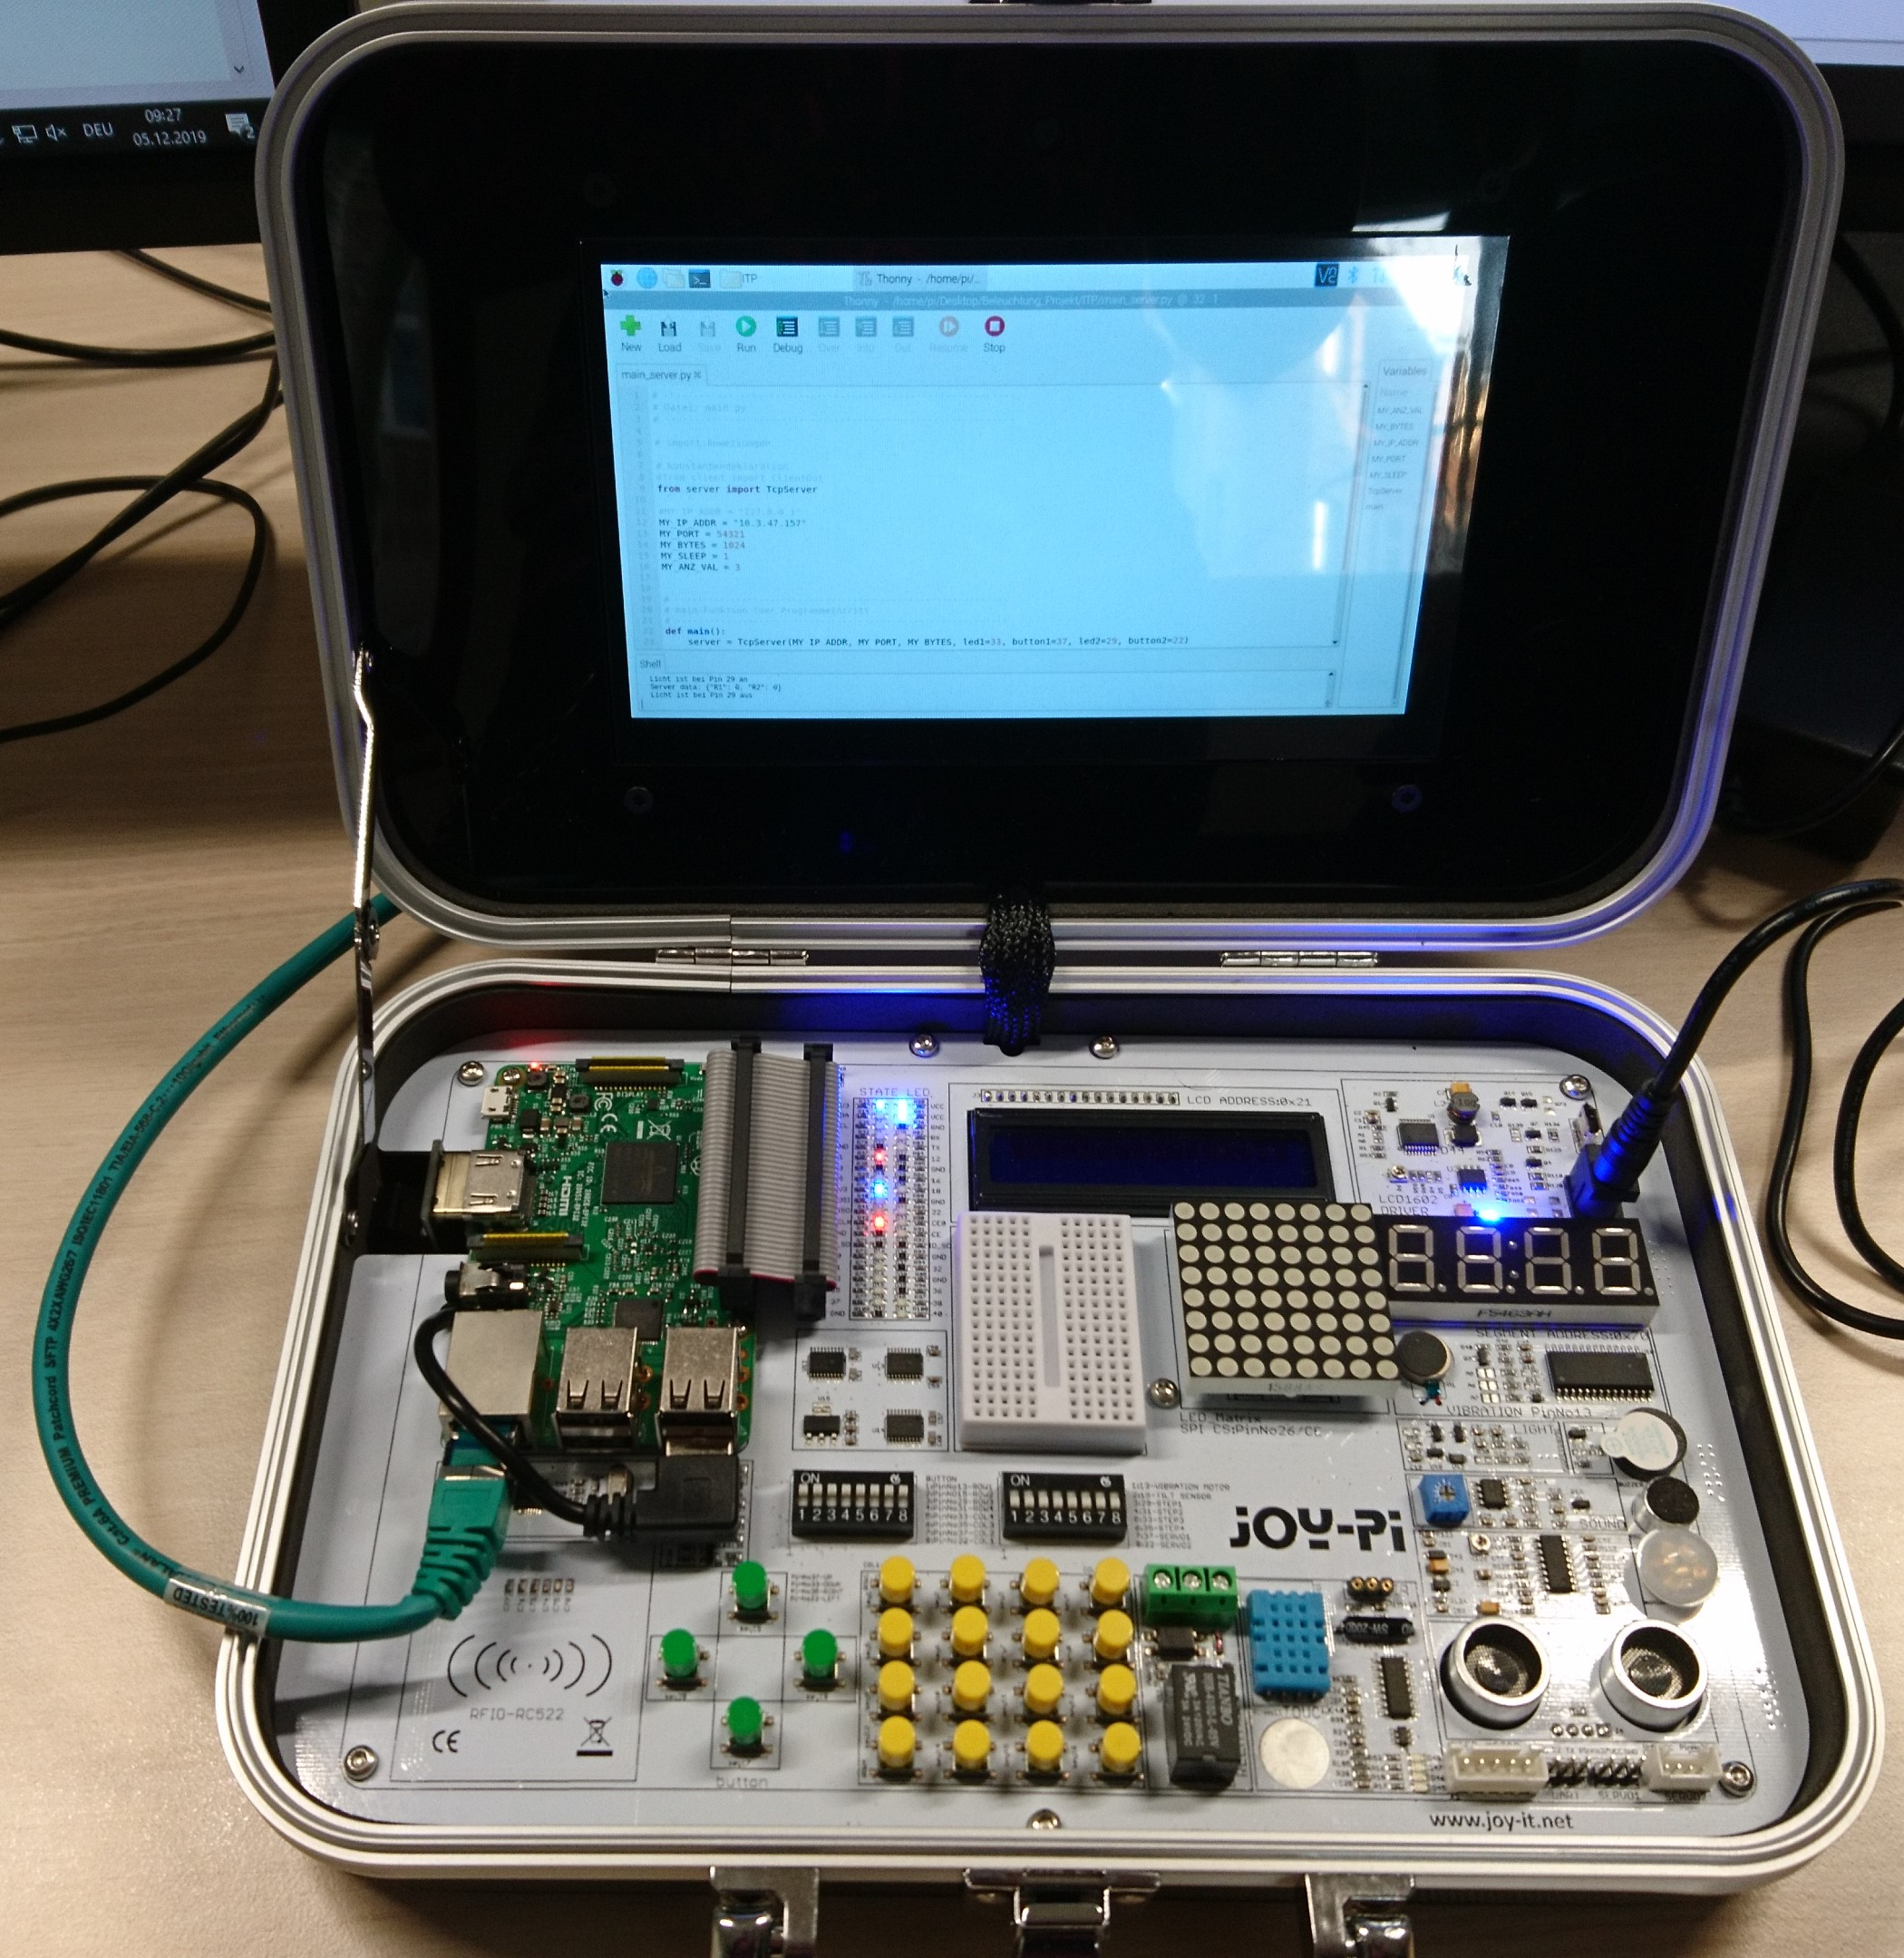
\includegraphics[width=10cm,height=10cm]{./_bilder/koffer.jpg} % 80-Prozent der Textbreite, nur PDF und PNG
\caption[Der Joy-Pi-Koffer]
{Der Joy-Pi-Koffer}
% [...] ist für das Abbildungsverzeichnis ohne Fußnote, {...} Beschriftung mit Fußnote (\footnotetext{...})
\label{fig:koffer}
} % schliesst \centering
\end{figure} % schliesst die Umgebung \begin{figure}
\section{Raspberry Pi}\label{sec:Raspberrypi}
Der Raspberry Pi ist ein kleiner Computer, der auf dem Joy-Pi montiert ist (siehe Abbildung \ref{fig:raspi}). Es gibt verschiedene Versionen des Raspberry Pi. In diesem Projekt wird der Raspberry Pi 3 B verwendet auf dem das Linux-Betriebssystem Raspbian installiert ist. Eine Programmierumgebung für Python mit dem Namen Thonny ist vorinstalliert. Es ist eine sehr einfach gehaltene Umgebung ohne viele Extras. Sie dient zur schnellen Programmierung, bietet allerdings wenig Unterstützung bei Problemen. Die technischen Daten des Raspberry Pi, wie Prozessorleistung etc. sind hier \cite{latex:raspberrypi} nachzulesen.
\begin{figure}[H] % H: figure wird an dieser Stelle eingefügt
	\centering{ % der Inhalt von figure wird zentriert ausgerichtet
		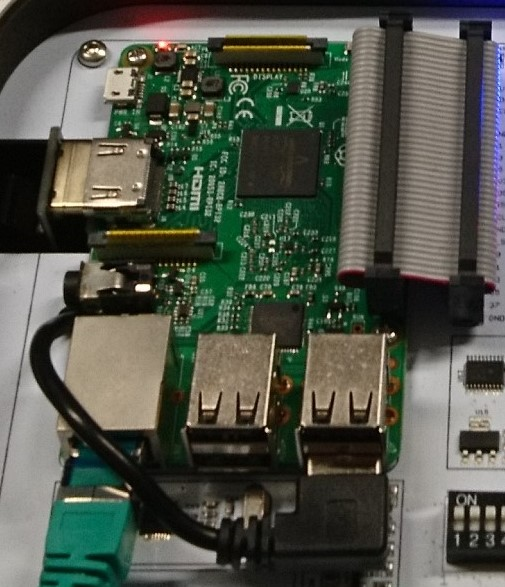
\includegraphics[width=5cm,height=5cm]{./_bilder/raspi.jpg} % 80-Prozent der Textbreite, nur PDF und PNG
		\caption[Der Raspberry-Pi 3 B]
		{Der Raspberry Pi 3 B}
		% [...] ist für das Abbildungsverzeichnis ohne Fußnote, {...} Beschriftung mit Fußnote (\footnotetext{...})
		\label{fig:raspi}
	} % schliesst \centering
\end{figure} % schliesst die Umgebung \begin{figure}
\section{Sensoren und Aktoren}
Wie schon erwähnt besteht der Koffer aus diversen Sensoren und Aktoren. In zwei Unterkapiteln wird erläutert welche Sensoren und Aktoren verbaut sind und kurz erklärt, wie sie funktionieren. Mit folgender Grafik \ref{fig:SuA} wird gezeigt welche Bauteile sich auf dem Koffer befinden. Die Bauteile sind blau und rot markiert. Blau für die Sensoren und rot für die Aktoren. Es gibt auf dem Bild zwei Nummerierungen, die in unterschiedlichen Farben aufgeführt sind, um Verwechslungen zwischen Sensoren und Aktoren zu vermeiden.
\begin{figure}[H] % H: figure wird an dieser Stelle eingefügt
\centering{ % der Inhalt von figure wird zentriert ausgerichtet
	%[width=14.5cm,height=8.2cm]
\includegraphics[width=0.9\textwidth]{./_bilder/Sensoren_Aktoren.png} % 80-Prozent der Textbreite, nur PDF und PNG
\caption[Sensoren und Aktoren des Joy-Pi]
{Sensoren und Aktoren des Joy-Pi}
% [...] ist für das Abbildungsverzeichnis ohne Fußnote, {...} Beschriftung mit Fußnote (\footnotetext{...})
\label{fig:SuA}
} % schliesst \centering
\end{figure} % schliesst die Umgebung \begin{figure}

\subsection{Sensoren}\label{sec:sensoren}

In diesem Unterkapitel werden die Sensoren behandelt. Mithilfe der folgenden Tabelle werden Name und Funktion der Sensoren erläutert. Die Nummerierung stammt aus Abbildung \ref{fig:SuA}.
\begin{longtable}{|L{2cm}|C{4.5cm}|C{7.5cm}|}
	\hline \textbf{Nummer} & \textbf{Sensor} &  \textbf{Funktion} \endfirsthead
	\hline \textbf{Nummer} & \textbf{Sensor} &  \textbf{Funktion}  \endhead
	\hline  1 & RFID-Modul & Zum Scannen eines RFID-Tags \\ 
	\hline  2 & Buttons mit \gls{ac:LED} & Signal durch Tasten erzeugen \\ 
	\hline  3 & Buttons ohne \gls{ac:LED} & Signal durch Tasten erzeugen \\ 
	\hline  4 & Berührungssensor & Signal durch Berührung erzeugen \\ 
	\hline  5 & Luftfeuchtigkeits-/Temperaturfühler & Kann die Luftfeuchtigkeit und Temperatur der Umgebung messen  \\ 
	\hline  6 & Ultraschallsensor & Wird zur Abstandsmessung verwendet \\ 
	\hline  7 & Bewegungssensor & Erkennt Bewegung in der Umgebung \\ 
	\hline  8 & Schallsesnor & Erkennt Geräusche in der Umgebung\\
	\hline  9 & Potentiometer & Ein per Hand einstellbarer Widerstand\\ 
	\hline 
	\caption{Tabelle zur Auflistung der Sensoren \label{tab:Sensoren}}
\end{longtable} 
\subsection{Aktoren}\label{sec:aktoren}

In diesem Unterkapitel werden die Aktoren behandelt. Mithilfe der folgenden Tabelle werden Name und Funktion dieser erläutert. Die Nummerierung stammt aus Abbildung \ref{fig:SuA}.

\begin{longtable}{|L{2cm}|C{4.5cm}|C{7.5cm}|}
	\hline \textbf{Nummer} & \textbf{Aktor} &  \textbf{Funktion} \endfirsthead
	\hline \textbf{Nummer} & \textbf{Aktor} &  \textbf{Funktion}  \endhead
	\hline  1 & \gls{ac:LED}s & Anzeigen von Signalen durch Leuchtzustand \\ 
	\hline  2 & \gls{ac:LCD}-Anzeige & Anzeigen von Daten (gute Auflösung) \\ 
	\hline  3 & \gls{ac:LED}-Matrix & Anzeigen von Daten (schlechte Auflösung) \\ 
	\hline  4 & Siebensegment-Anzeige & Analoge Werte können angezeigt werden \\ 
	\hline  5 & Buzzer & Erzeugt Töne bei Aktivierung  \\ 
	\hline  6 & Anschluss Servomotor & Schrittweise einstellbarer Motor \\ 
	\hline  7 & Anschluss Schrittmotor & Motor mit hoher Drehzahl \\ 
	\hline  8/(9) & Relais mit Anschlüssen & Öffnen und Schließen von elektrischen Schaltkreisen\\
	\hline  10 & Vibrationsmodul & Vibriert bei Aktivierung\\ 
	\hline 
	\caption{Tabelle zur Auflistung der Aktoren \label{tab:Aktoren}}
\end{longtable}
Zusätzlich können die Informationen zu Sensoren und Aktoren in der Anleitung des Joy-Pi nachgelesen werden \cite{latex:anleitung}.
\section{Besonderheiten des Joy-Pi}
Der Joy-Pi hat diverse Besonderheiten, die in diesem Teil des Berichts erläutert werden. Es wird auf Themen wie Logik, Board-Nummern und die Python-Version eingegangen.

\subsection{Logik}\label{sec:Logik}
In diesem Projekt werden neben einer grafischen Oberfläche und einer \gls{ac:tcpip}-Verbindung auch Hardware-Komponenten programmiert. Diese Komponenten erzeugen und verarbeiten Signale, die korrekt interpretiert und verarbeitet werden müssen. Mithilfe von Tastern (Hardware-Eingänge) sollen \gls{ac:LED}s (Hardware-Ausgänge) an- und ausgeschaltet werden. Daraus folgt, dass die Ein- und Ausgänge digital sind. Nun ist bei dem Joy-Pi darauf zu achten, dass die digitalen Ein- und Ausgänge mit einer negativen Logik arbeiten. Somit wird die Logik vom Board vorgegeben und nicht vom Raspberry Pi. Das bedeutet, dass wenn zum Beispiel an einem Ausgang eine positive Spannung anliegt (\textit{High-Signal}), wird die \gls{ac:LED} nicht ein- sondern ausgeschaltet. Um sie einzuschalten, müsste die \gls{ac:LED} den Wert \textit{Low} erhalten (niedriger Spannungspegel). Bei den Eingängen funktioniert dies auf die gleiche Art, allerdings werden hierbei nur die Flanken von ihnen abgefragt(näheres wird in Kapitel 3 beschrieben).

\subsection{Board-Nummern}
Die Bauteile des Joy-Pi sind an Pins angeschlossen, welche auf dem Board mit Nummern versehen sind. Diese Nummerierung unterscheidet sich von der in der Anleitung. In diesem Projekt wird nicht mit den Nummern in der Anleitung gearbeitet, sondern mit den Board-Nummern. Wenn also im Quelltext eine Pin-Nummer zugewiesen wird, muss auf dem Board nachgeschaut werden, um welchen Pin es sich handelt. Die Abbildung \ref{fig:board} zeigt wie die Nummerierung dargestellt ist. Es sind Nummern, die neben den jeweiligen Bauteilen angebracht sind. Hier werden beispielsweise die \gls{ac:LED}s gezeigt.
\begin{figure}[H] % H: figure wird an dieser Stelle eingefügt
	\centering{ % der Inhalt von figure wird zentriert ausgerichtet
		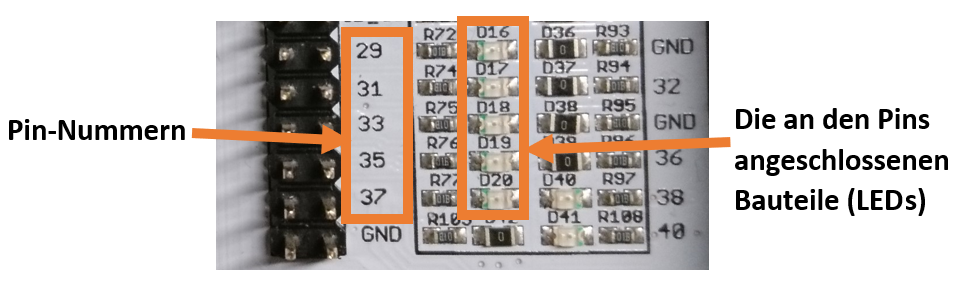
\includegraphics[width=14cm,height=4cm]{./_bilder/Board_Nummern.png} % 80-Prozent der Textbreite, nur PDF und PNG
		\caption[Pin-Nummern und deren Bauteile]
		{Pin-Nummern und deren Bauteile}
		% [...] ist für das Abbildungsverzeichnis ohne Fußnote, {...} Beschriftung mit Fußnote (\footnotetext{...})
		\label{fig:board}
	} % schliesst \centering
\end{figure} % schliesst die Umgebung
Aus der Abbildung geht nicht hervor, dass es Pins gibt, die an mehreren Bauteilen angeschlossen sind. Zum Beispiel Pin 37 aus Abbildung \ref{fig:board}, welcher zum einen an die \gls{ac:LED} angeschlossen ist, aber auch an einem Taster.
\subsection{Python-Version}
Die Programmiersprache Python ist eine interpretierbare Sprache und hat verschiedene Versionen. Je nach Version unterscheidet sich die Syntax (Grammatik der Programmiersprache), außerdem bieten aktuellere Versionen neue Funktionen mit denen gearbeitet werden kann. In diesem Projekt wird Python 3.7.3 zur Programmierung genutzt. 

%--------------------------------------------------------------------------------
\chapter{Realisierung des Projektes}
Folgend wird die Umsetzung der zuvor geplanten Aspekte erläutert. 

\section{Ansteuerung der Sensoren und Aktoren}
Wie zuvor erwähnt wurde, soll eine \gls{ac:LED} durch einen Hardware-Taste ein- und ausgeschaltet werden können. Dies gelingt durch die Ansteuerung der Hardware-Pins des Raspberry Pis, welche \gls{ac:gpio} genannt werden. An diesen Pins sind Aktoren und Sensoren angeschlossen. Die Ansteuerung erfolgt in Python über die \gls{ac:gpio}-Bibliothek \cite{latex:gpio}. Sensoren sind im Rahmen dieses Projektes die Hardware-Tasten des Joy-Pi, welche in Abbildung \ref{fig:button} dargestellt sind. In Abbildung \ref{fig:LED} werden die verwendeten Aktoren, hier \gls{ac:LED}s, gezeigt. 

\begin{figure}[H] % H: figure wird an dieser Stelle eingefügt
	\centering{ % der Inhalt von figure wird zentriert ausgerichtet
		\begin{minipage}[t]{0.45\linewidth}
			\centering{ % der Inhalt von figure wird zentriert ausgerichtet
				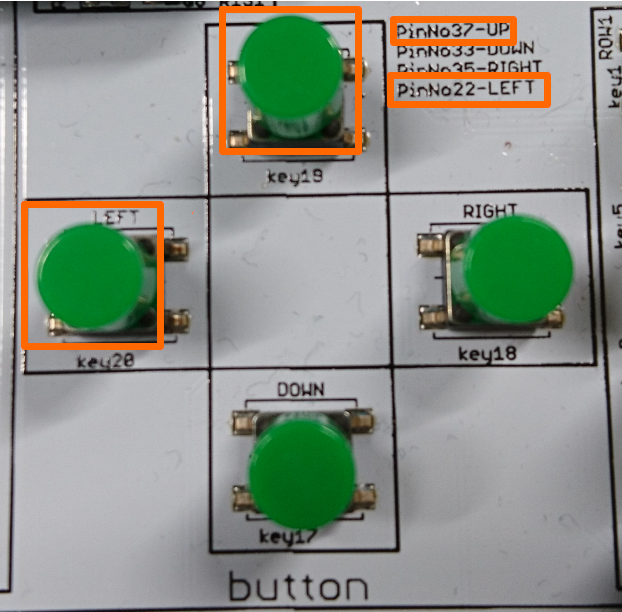
\includegraphics[width=7cm,height=7cm]{./_bilder/Buttons_Beschriftet.png} % 80-Prozent der Textbreite, nur PDF und PNG
				\caption[Im Projekt verwendete Tasten des Joy-Pi]
				{Im Projekt verwendete Tasten des Joy-Pi}
				% [...] ist für das Abbildungsverzeichnis ohne Fußnote, {...} Beschriftung mit Fußnote (\footnotetext{...})
				\label{fig:button}
			} % schliesst \centering
		\end{minipage}\hfill
		\begin{minipage}[t]{0.45\linewidth}
			\centering{ % der Inhalt von figure wird zentriert ausgerichtet
				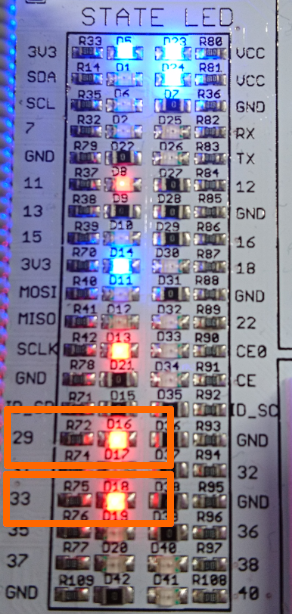
\includegraphics[width=3.5cm,height=8cm]{./_bilder/LED_beschriftet.png} % 80-Prozent der Textbreite, nur PDF und PNG
				\caption[Im Projekt verwendete LEDs des Joy-Pi]
				{Im Projekt verwendete LEDs des Joy-Pi}
				% [...] ist für das Abbildungsverzeichnis ohne Fußnote, {...} Beschriftung mit Fußnote (\footnotetext{...})
				\label{fig:LED}
			} % schliesst \centering	
		\end{minipage}\hfill
	} % schliesst \centering
\end{figure} % schliesst die Umgebung \begin{figure}

Es werden die markierten Tasten und \gls{ac:LED}s verwendet. Die obere Taste ist an Pin 37 angeschlossen (vgl. Abbildung \ref{fig:button}) und soll die Beleuchtung im Raum 1 steuern. Sie wird im Folgenden Text \textit{Taste 1} genannt. Die linke Taste soll das Licht in Raum 2 über Pin 22 (vgl. Abbildung \ref{fig:button}) ansteuern und wird daher im weiterem Verlauf \textit{Taste 2} benannt. Die obere Leuchtdiode ist an Pin 29 angeschlossen und simuliert das Licht des ersten Raumes. Die untere \gls{ac:LED} stellt die Beleuchtung des zweiten Raumes dar und erhält über Pin 33 ihr Signal (siehe Abbildung \ref{fig:LED}). Der Aktor des ersten Raumes wird im Textverlauf \textit{LED 1}, der des zweiten Raumes \textit{LED 2} genannt. Über die \gls{ac:gpio} Klasse können Zustände dieser Pins eingelesen und Signaländerungen ausgegeben werden.\\[0,2cm]

Der Quelltext \ref{lst:qbutton} zeigt, wie in Python ein Tastendruck eingelesen wird. Nachdem in der 2. Zeile des Quelltextes \ref{lst:qbutton} einer Variablen \texttt{button1\_pin} die Pin-Nummer \texttt{37} (\textit{Taste 1}) der Hardware-Pins zugeordnet wurde, wird in Zeile 5 diese Pin-Nummer der Methode \texttt{setup} der \gls{ac:gpio} Klasse übergeben und über \texttt{GPIO.IN} als Eingang festgelegt. Der Parameter \texttt{GPIO.PUD\_DOWN} definiert an dem übergebenen Pin einen Pulldown-Widerstand. Bei geöffnetem Kontakt wird also die Spannung am Pin auf Masse gezogen und erzeugt so ein eindeutiges LOW-Signal \cite{latex:pulld}. In Zeile 8 des Quelltextes  \ref{lst:qbutton} kann über die Methode \texttt{add\_event\_detect} definiert werden, welche Aktion bei Betätigung der Taste durchgeführt werden soll. Dabei wird die Pin-Nummer, die Flanke bei der die Aktion durchgeführt werden soll (hier die steigende Flanke), die Callback-Funktion und eine Zeit übergeben. Die Callback-Funktion ist dabei die Funktion, die bei Betätigung ausgeführt wird (hier: \texttt{button1\_interrupt}). Die Zeit von $500$ $ms$ entprellt die Taste und verhindert so unerwünschte Signale. Die Funktion \texttt{button1\_interrupt} soll \textit{LED 1} steuern. Der Quelltext lässt sich dann auf \textit{Taste 2} übertragen.\\

\begin{lstlisting}[style=python, caption=Python-Code zum Einlesen des Tastenzustandes, label=lst:qbutton]
#Erstellen einer Variablen 
button1_pin=37
 
#Festlegung als Eingang
GPIO.setup(button1_pin, GPIO.IN, pull_up_down=GPIO.PUD_DOWN)

#Ereignis bei Betaetigung des Buttons
GPIO.add_event_detect(button1_pin, GPIO.RISING, callback=button1_interrupt, bouncetime=500)
\end{lstlisting}



\newpage

Wie eine \gls{ac:LED} in Python angesteuert wird, zeigt Quelltext \ref{lst:qLED}. Pin \texttt{33} (\textit{LED 1}) wird in Zeile 2 des Quelltextes \ref{lst:qLED} die Variable \texttt{LED1\_pin} zugewiesen. Folgend wird in Zeile 5 diese Variable über \texttt{GPIO.OUT} als Ausgang festgelegt. Aufgrund der internen Verschaltung wird die \gls{ac:LED} in negativer Logik angesprochen (Näheres ist in Kapitel \ref{sec:Logik} erklärt). Aus diesem Grund wird in Zeile 8 über \texttt{GPIO.LOW} eine Spannung an den \texttt{LED\_pin} angelegt: Die \gls{ac:LED} leuchtet. Über \texttt{GPIO.HIGH} wird dies in Zeile 9 wieder rückgängig gemacht (siehe auch Kapitel \ref{sec:Logik}). Auch hier lässt sich der Quelltext auf die zweite Leuchtdiode (\textit{LED 2}) übertragen (vgl. Abbildung \ref{fig:LED}).\\[0.2cm]

\begin{lstlisting}[style=python, caption=Python-Code zur Ansteuerung einer LED, label=lst:qLED]
#Erstellen einer Variablen
LED1_pin=33

#Festlegung als Ausgang
GPIO.setup(LED1_pin, GPIO.OUT)

#Ansteuerung
GPIO.output(LED_pin, GPIO.LOW)
GPIO.output(LED_pin, GPIO.HIGH)

\end{lstlisting}

Die oben genannten Errungenschaften können nun programmiertechnisch so verknüpft werden, dass mit den Tasten die \gls{ac:LED}s angesteuert werden. Nun ist es möglich mit \textit{Taste 1} \textit{LED 1} und mit \textit{Taste 2}  \textit{LED 2} anzusteuern.
 
\section{Grafische Oberfäche mit Tkinter}
\label{sec:gui}
Die Ansteuerung der \gls{ac:LED}s soll nun auch über eine grafische Oberfläche möglich sein. Diese soll zunächst auf dem Raspberry Pi aufgerufen werden können. Um das \gls{ac:gui} zu erstellen, wird die Python-Bibliothek Tkinter \cite{latex:tkinter} verwendet.
In Abbildung \ref{fig:gui2} ist diese grafische Oberfläche dargestellt. Jeder Raum besitzt jeweils eine Taste zum ein- und ausschalten sowie eine \gls{ac:LED}-Status-Anzeige. Diese soll darstellen, ob die Leuchtdiode auf dem Joy-Pi eingeschaltet ist oder nicht.

% Dabei ist diese in zwei Teile aufgeteilt, in denen sich jeweils die Schaltflächen zum ein- und ausschalten der LEDs befinden. Zusätzlich ist in jedem Abschnitt eine LED-Status-Anzeige vorhanden. 

\begin{figure}[H] % H: figure wird an dieser Stelle eingefügt
	\centering{ % der Inhalt von figure wird zentriert ausgerichtet
		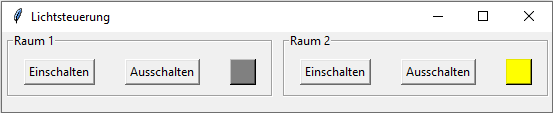
\includegraphics[width=14cm,height=3cm]{./_bilder/Gui_1-aus_2-an.png} % 80-Prozent der Textbreite, nur PDF und PNG
		\caption[Grafische Oberfläche programmiert mit Python und Tkinter]
		{Grafische Oberfläche programmiert mit Python und Tkinter}
		% [...] ist für das Abbildungsverzeichnis ohne Fußnote, {...} Beschriftung mit Fußnote (\footnotetext{...})
		\label{fig:gui2}
	} % schliesst \centering
\end{figure} % schliesst die Umgebung

In Quelltext \ref{lst:qgui} ist die programmiertechnische Beschreibung des \gls{ac:gui} dargestellt. Dabei wird in Zeilen 3 bis 5 ein Fenster mit der Überschrift \texttt{Lichtsteuerung} und den Maßen \texttt{550 px $\cdot$ 80 px} erstellt. Der erste Rahmen, der die Schaltflächen für Raum 1 beinhaltet (vgl. Abbildung \ref{fig:gui2}) wird in den Zeilen 7 und 8 erstellt. Die Schaltfläche zum Einschalten wird in Zeilen 10 und 11, die zum Ausschalten in Zeilen 13 und 14 generiert. Zusätzlich entsteht durch die 16. und 17. Zeile eine Schaltfläche, die neben der Taste zum Ausschalten positioniert wird, um den Zustand der \gls{ac:LED}s anzuzeigen. Diese Schritte werden für Raum 2 in Zeilen 19-30 wiederholt.\\[0,2cm]

\begin{lstlisting}[style=python, caption=Python-Code der verwendeten Dictionaries, label=lst:qgui]
import tkinter as tk

window = tk.Tk()
window.title("Lichtsteuerung")
window.geometry("550x80")

lbl= tk.LabelFrame(window, text="Raum 1", width=250, height=80)
lbl.grid(row=0, column=0, columnspan=2, sticky="W", padx=5, pady=0, ipadx=0, ipady=0)

an_btn = tk.Button(lbl, text="Einschalten", command=callback_an_raum1)
an_btn.grid(column=0, row=1, padx=15, pady=10)

aus_btn = tk.Button(lbl, text="Ausschalten", command=callback_aus_raum1)
aus_btn.grid(column=1, row=1, padx=15, pady=10)

anzeige1 = tk.Button(lbl, text="     ", bg="grey", command="")
anzeige1.grid(column=2, row=1, padx=15, pady=10)

lbl2= tk.LabelFrame(window, text="Raum 2", width=250, height=80)
lbl2.grid(row=0, column=2, columnspan=2, sticky="W", padx=5, pady=0, ipadx=0, ipady=0)

an_btn = tk.Button(lbl2, text="Einschalten", command=callback_an_raum2)
an_btn.grid(column=0, row=1, padx=15, pady=10)

aus_btn = tk.Button(lbl2, text="Ausschalten", command=callback_aus_raum2)
aus_btn.grid(column=1, row=1, padx=15, pady=10)

anzeige2 = tk.Button(lbl2, text="     ", bg="grey", command="")
anzeige2.grid(column=2, row=1, padx=15, pady=10)
\end{lstlisting}

\newpage

Das Schalten der Tasten eines Raumes bewirkt die Farbänderung der \gls{ac:LED}-Status-Anzeige. Diese wird beim Einschalten gelb und beim Ausschalten grau (vgl. Abbildung \ref{fig:gui2}). Durch die Callback-Funktion, welche durch den Parameter \texttt{command} übergeben wird, kann dies erreicht werden (siehe Quelltext \ref{lst:qLED} Zeilen 10, 13, 22 und 25). Um nun auch die Leuchdioden auf dem Joy-Pi mit den Schaltflächen der \gls{ac:gui} ansteuern zu können, wird in die jeweilige Callback-Funktion der Befehl zum Schalten der \gls{ac:LED}s eingegeben.\\[0,2cm]
Nun können durch die grafische Oberfläche die Leuchtdioden ein- bzw. ausgeschaltet und der Zustand der \gls{ac:LED}s angezeigt werden.

\section{TCP/IP-Verbindung}
Die Ansteuerung der Leuchtdioden kann nun über die grafische Oberfläche auf dem Raspberry Pi erfolgen. Das nächste Ziel ist, das \gls{ac:gui} auf einem anderen Computer zu starten, um von dort die Befehle an den Raspberry Pi zu übertragen. Damit dies gelingt, soll die Verbindung über \gls{ac:tcpip} hergestellt werden. Die \gls{ac:tcpip}-Verbindung  gehört zu der Familie der Netzwerk-Protokolle und ermöglicht einen Austausch von Datenpaketen über eine Netzwerkverbindung  \cite{latex:tcpip}.
In Abbildung \ref{fig:tcpip} wird diese Verbindung schematisch dargestellt. Dabei soll der Joy-Pi und damit der Raspberry Pi die Aufgabe des Servers übernehmen. Der externe Computer stellt den Client dar und soll sich mit dem Server verbinden. Dafür wird dem Client eine Adresse vorgegeben, die auf dem Prinzip des \gls{ac:ip} beruht. Es ist die \gls{ac:ip}-Adresse des Raspberry Pi. Dieser wartet darauf, dass sich ein Client mit ihm verbindet. Anschließend können vom Raspberry Pi Informationen über die Tasten und Zustände der \gls{ac:LED}s an den externen Computer gesendet werden. Dieser wiederum sendet die Signale der Schaltflächen an den Server. Dies geschieht gleichzeitig.
\begin{figure}[H] % H: figure wird an dieser Stelle eingefügt
	\centering{ % der Inhalt von figure wird zentriert ausgerichtet
		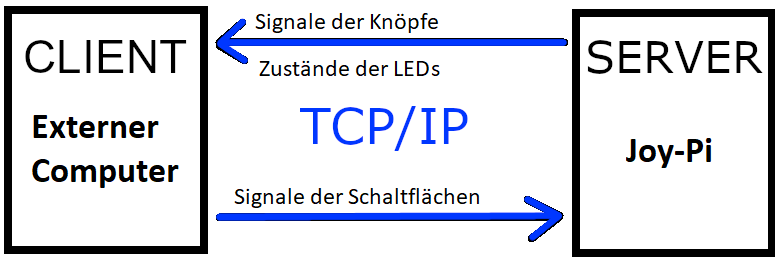
\includegraphics[width=10.5cm,height=3.7cm]{./_bilder/Kommunikation_1.png} % 80-Prozent der Textbreite, nur PDF und PNG
		\caption[Datenaustausch zwischen externem Computer und Joy-Pi]
		{Datenaustausch zwischen externem Computer und Joy-Pi über \gls{ac:tcpip}-Verbindung}
		% [...] ist für das Abbildungsverzeichnis ohne Fußnote, {...} Beschriftung mit Fußnote (\footnotetext{...})
		\label{fig:tcpip}
	} % schliesst \centering
\end{figure} % schliesst die Umgebung \begin{figure}


Die Verbindung wird in Python unter Verwendung des Moduls \texttt{json} \cite{latex:json} umgesetzt. \gls{ac:JSON} ist eine Syntax, die zum Datenaustausch oder zur Datenspeicherung dient \cite{latex:json2}. Dabei ähnelt diese Syntax sehr dem der Python-Dictionaries. Durch Funktionen aus dem \texttt{json}-Modul können diese Dictionaries ausgelesen oder erzeugt werden \cite{latex:kofler}. In diesem Projekt werden Dictionaries verwendet, um die Zustände der \gls{ac:LED}s, der Tasten und der Schaltflächen des \gls{ac:gui} zu übertragen. Dieser Datenaustausch wird durch die Python-Bibliothek \texttt{socket} \cite{latex:socket} ermöglicht.
Die Dictionaries werden durch die Methode \texttt{json.dumps} in Strings umgewandelt \cite{latex:kofler} und können über \texttt{encode()} (eine Funktion der Klasse \texttt{socket}) als Byte-Kette abgesendet werden \cite{latex:socket2}.
Beim Empfänger wird diese Byte-Kette über \texttt{decode()} zurück in einen String umgewandelt, um daraus anschließend mit \texttt{json.loads}  ein Dictionary zu erzeugen \cite{latex:kofler}.
Folgend kann ein Auslesen und Auswerten der Daten erfolgen.\\

%----------------------------------------------------------------------
\chapter{Ergebnis}
Das Ergebnis des Projektes wird im Folgenden erläutert.

\section{Hardware}
Im Projekt wurde ein Computer verwendet (vgl. Abbildung \ref{fig:hardware} links), der über das Netzwerk mit dem Raspberry Pi (vgl. Abbildung \ref{fig:hardware} rechts) verbunden ist. An diesem sind sowohl die verwendeten \gls{ac:LED}s (rot markiert) als auch die genutzten Tasten (blau markiert) angeschlossen.
\begin{figure}[H] % H: figure wird an dieser Stelle eingefügt
	\centering{ % der Inhalt von figure wird zentriert ausgerichtet
		\includegraphics[width=1\linewidth]{./_bilder/Hardware.png} % 80-Prozent der Textbreite, nur PDF und PNG
		\caption[Projektaufbau mit genutzter Hardware]
		{Projektaufbau mit genutzter Hardware}
		% [...] ist für das Abbildungsverzeichnis ohne Fußnote, {...} Beschriftung mit Fußnote (\footnotetext{...})
		\label{fig:hardware}
	} % schliesst \centering
\end{figure} % schliesst die Umgebung \begin{figure}
\newpage
In Abbildung \ref{fig:LEDstatus} werden die unterschiedlichen Zustände gezeigt, die \textit{LED 1} und \textit{LED 2} annehmen können. Wird keine der beiden Tasten gedrückt, leuchtet auch keine der \gls{ac:LED}s (vgl. linkes Bild aus Abbildung \ref{fig:LEDstatus}). Wird \textit{Taste 1} betätigt, wird \textit{LED 1} eingeschaltet (vgl. mittleres linkes Bild aus Abbildung \ref{fig:LEDstatus}). Sobald anschließend \textit{Taste 2} gedrückt wird, leuchtet zusätzlich noch \textit{LED 2} (vgl. mittleres rechtes Bild aus Abbildung \ref{fig:LEDstatus}). Wird \textit{Taste 1} erneut gedrückt erlischt \textit{LED 1} und nur noch \textit{LED 2} bleibt eingeschaltet (vgl. rechtes Bild aus Abbildung \ref{fig:LEDstatus}). Diese erlischt, sobald \textit{Taste 2} erneut gedrückt wird. Diese Schaltvorgänge können beliebig oft und in beliebiger Reihenfolge durchgeführt werden.

\begin{figure}[H] % H: figure wird an dieser Stelle eingefügt
	\centering{ % der Inhalt von figure wird zentriert ausgerichtet
		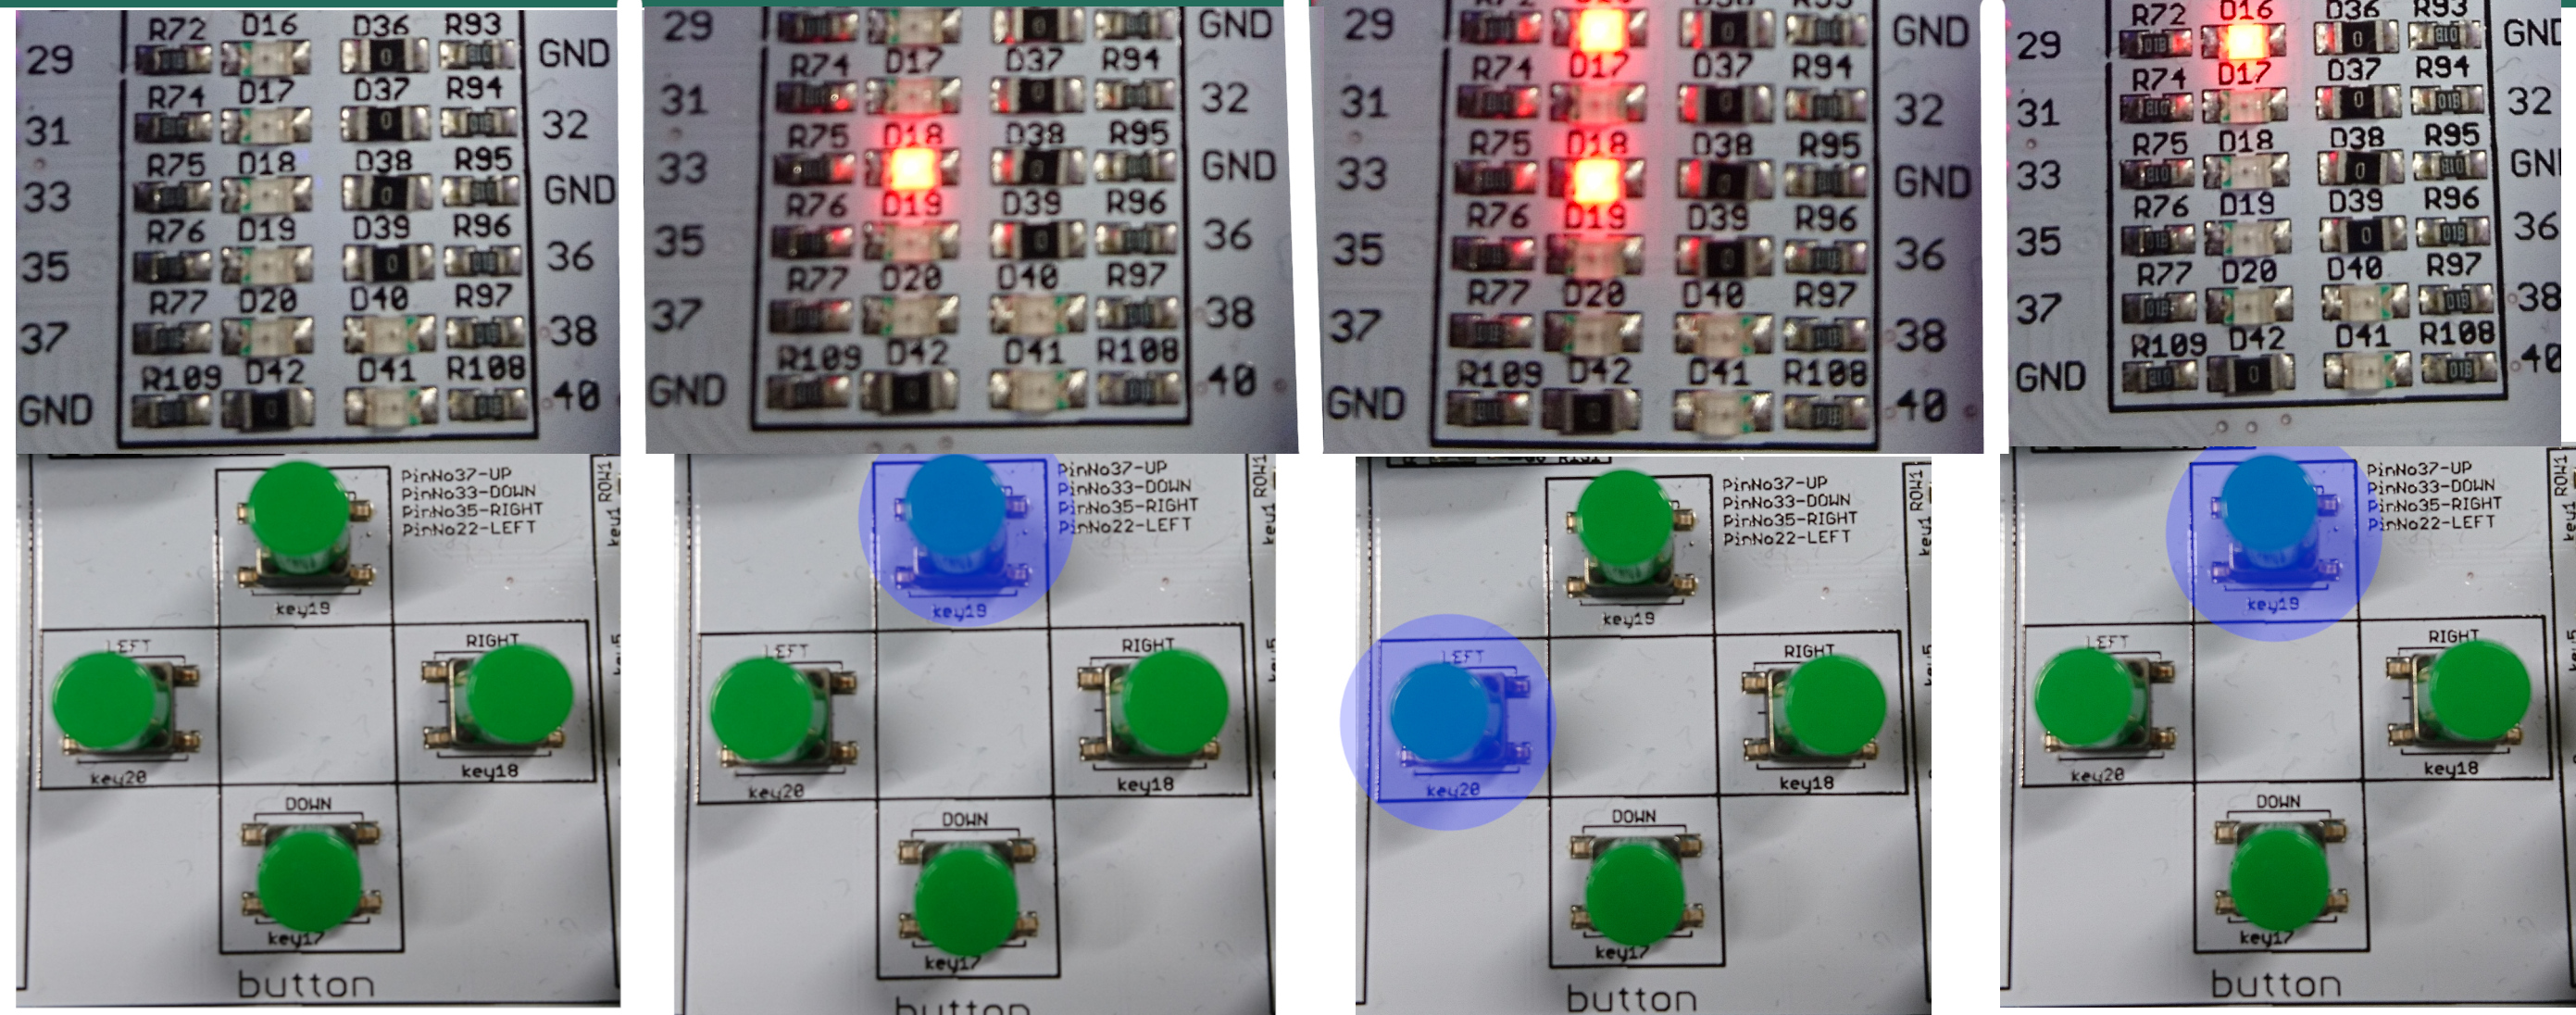
\includegraphics[width=1\linewidth]{./_bilder/LEDZustand.jpg} % 80-Prozent der Textbreite, nur PDF und PNG
		\caption[Zustände der LEDs]
		{Zustände der LEDs}
		% [...] ist für das Abbildungsverzeichnis ohne Fußnote, {...} Beschriftung mit Fußnote (\footnotetext{...})
		\label{fig:LEDstatus}
	} % schliesst \centering
\end{figure} % schliesst die Umgebung \begin{figure}

\section{Grafische Oberfläche}
Um die \gls{ac:LED}s auch von einem anderen Computer als den Raspberry Pi aus steuern zu können, wurde eine grafische Oberfläche programmiert (vgl. Kapitel \ref{sec:gui}). Diese kann nun über einen externen Rechner aufgerufen werden. In den folgenden Abbildungen ist das \gls{ac:gui} bei unterschiedlichen Betätigungen dargestellt.\\[0.2cm]
In Abbildung \ref{fig:gui1an} wird über die grafische Oberfläche \textit{Raum 1} eingeschaltet. Dabei wird über die \gls{ac:LED}-Status-Anzeige mitgeteilt, dass \textit{LED 1} auf dem Joy-Pi leuchtet. Wird anschließend in Abbildung \ref{fig:gui1aus} wieder ausgeschaltet, erlischt \textit{LED 1} und die Schaltfläche der Status-Anzeige wird grau. 

\begin{figure}[H] % H: figure wird an dieser Stelle eingefügt
	\centering{ % der Inhalt von figure wird zentriert ausgerichtet
		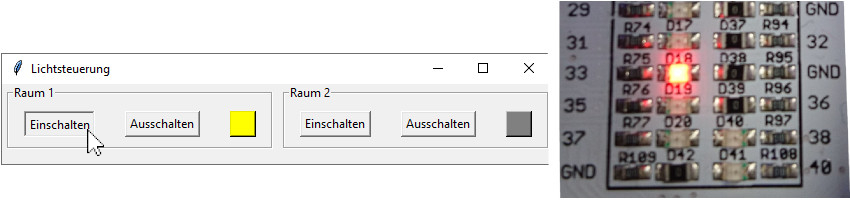
\includegraphics[width=1\linewidth]{./_bilder/GUI1an.jpg} % 80-Prozent der Textbreite, nur PDF und PNG
		\caption[Grafische Oberfläche bei Betätigung der Einschalt-Taste des ersten Raumes]
		{Grafische Oberfläche bei Betätigung der Einschalt-Taste des ersten Raumes}
		% [...] ist für das Abbildungsverzeichnis ohne Fußnote, {...} Beschriftung mit Fußnote (\footnotetext{...})
		\label{fig:gui1an}
	} % schliesst \centering
\end{figure} % schliesst die Umgebung \begin{figure}

\begin{figure}[H] % H: figure wird an dieser Stelle eingefügt
	\centering{ % der Inhalt von figure wird zentriert ausgerichtet
		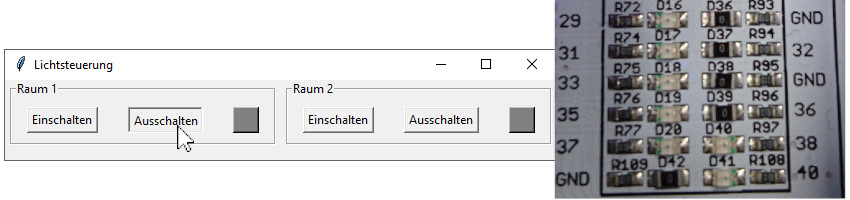
\includegraphics[width=1\linewidth]{./_bilder/GUI1aus.jpg} % 80-Prozent der Textbreite, nur PDF und PNG
		\caption[Grafische Oberfläche bei Betätigung der Ausschalt-Taste des ersten Raumes]
		{Grafische Oberfläche bei Betätigung der Ausschalt-Taste des ersten Raumes}
		% [...] ist für das Abbildungsverzeichnis ohne Fußnote, {...} Beschriftung mit Fußnote (\footnotetext{...})
		\label{fig:gui1aus}
	} % schliesst \centering
\end{figure} % schliesst die Umgebung \begin{figure}

Genauso verhält es sich auch beim Ein- und Ausschalten der \textit{LED 2} des \textit{Raumes 2}. Beim Einschalten leuchtet \textit{LED 2} und die Status-Anzeige wird gelb  (vgl. Abbildung \ref{fig:gui2an}), beim Ausschalten erlischt \textit{LED 2} und der \gls{ac:LED}-Status wechselt auf grau (vgl. Abbildung \ref{fig:gui2aus}).

\begin{figure}[H] % H: figure wird an dieser Stelle eingefügt
	\centering{ % der Inhalt von figure wird zentriert ausgerichtet
		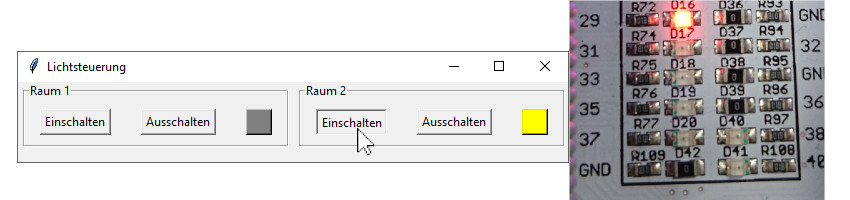
\includegraphics[width=1\linewidth]{./_bilder/GUI2an.jpg} % 80-Prozent der Textbreite, nur PDF und PNG
		\caption[Grafische Oberfläche bei Betätigung der Einschalt-Taste des zweiten Raumes]
		{Grafische Oberfläche bei Betätigung der Einschalt-Taste des zweiten Raumes}
		% [...] ist für das Abbildungsverzeichnis ohne Fußnote, {...} Beschriftung mit Fußnote (\footnotetext{...})
		\label{fig:gui2an}
	} % schliesst \centering
\end{figure} % schliesst die Umgebung \begin{figure}

\begin{figure}[H] % H: figure wird an dieser Stelle eingefügt
	\centering{ % der Inhalt von figure wird zentriert ausgerichtet
		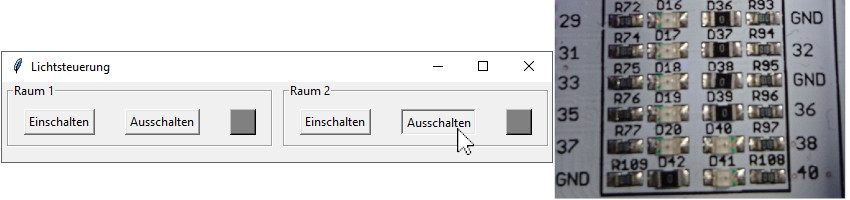
\includegraphics[width=1\linewidth]{./_bilder/GUI2aus.jpg} % 80-Prozent der Textbreite, nur PDF und PNG
		\caption[Grafische Oberfläche bei Betätigung der Ausschalt-Taste des zweiten Raumes]
		{Grafische Oberfläche bei Betätigung der Ausschalt-Taste des zweiten Raumes}
		% [...] ist für das Abbildungsverzeichnis ohne Fußnote, {...} Beschriftung mit Fußnote (\footnotetext{...})
		\label{fig:gui2aus}
	} % schliesst \centering
\end{figure} % schliesst die Umgebung \begin{figure}

Über die grafische Oberfläche können von einem externen Computer also die Leuchtdioden des Joy-Pi beliebig gesteuert werden. Dabei wird der aktuelle \gls{ac:LED}-Status auf dem \gls{ac:gui} angezeigt.  



\section{Verbindung}
Die Verbindung zwischen Raspberry Pi (Server) und dem externen Computer (Client) wurde mit einer Netzwerkverbindung über \gls{ac:tcpip} realisiert. Die Daten, die dabei ausgetauscht werden, sind in Dictionaries abgespeichert. Im Quelltext \ref{lst:qdic} sind diese Dictionaries dargestellt. Auf der Client-Seite wird das Dictionary \texttt{raeume} verwendet. Dabei werden den Schlüsselwörtern \texttt{R1} und \texttt{R2}, welche Raum 1 und Raum 2 darstellen, eine \texttt{0} zugewiesen, wenn ein Ausschalten seitens der grafischen Oberfläche erfolgt. Falls eingeschaltet wird, wird eine \texttt{1} zugeordnet. Ähnlich ist es bei dem Dictionary \texttt{LEDs\_state} auf der Server-Seite: Hier wird der Status von \textit{LED 1} und \textit{LED 2} festgehalten. Eine ausgeschaltete Leuchtdiode bewirkt die Zuweisung einer \texttt{0}, eine eingeschaltete die Zuweisung einer \texttt{1}. Im unten gezeigtem Quellttext \ref{lst:qdic} sind beide Räume ausgeschaltet und die \gls{ac:LED}s leuchten nicht.

\begin{lstlisting}[style=python, caption=Python-Code der verwendeten Dictionaries, label=lst:qdic]
#Dictionary auf der Client-Seite
raeume = {"R1": 0, "R2": 0}

#Dictionary auf der Server-Seite
LEDs_state = {"LED1": 0, "LED2": 0}
\end{lstlisting}

Wird auf der grafischen Oberfläche z.B. \textit{Raum 1} eingeschaltet, wird diese Information im Dictionary \texttt{raeume} abgespeichert und versendet. Sobald der Raspberry Pi den Datenstrom des Clients (externer Computer) ausgelesen hat, werden die Daten des Dictionaries \texttt{LEDs\_state} aktualisiert und die Funktion zum Einschalten von \textit{LED 1} ausgeführt. Da sich nun der Zustand der \gls{ac:LED} geändert hat, werden diese Daten zurück an den Client gesendet. Dieser aktualisiert wiederum sein Dictionary und führt die Funktion zum Einschalten der \gls{ac:LED}-Statusanzeige des ersten Raumes auf dem \gls{ac:gui} aus.\\
Wird auf dem Joy-Pi nun \textit{Taste 1} oder \textit{Taste 2} gedrückt, werden entsprechende \gls{ac:LED} geschaltet und der Raspberry Pi sendet das aktuelle Dictionary \texttt{LEDs\_state} zum externen Computer. Dieser wiederum ließt diese Daten aus und zeigt den neuen \gls{ac:LED}-Status auf dem \gls{ac:gui} an.
%----------------------------------------------------------------------
\chapter{Zusammenfassung und Ausblick}
%1-1,5 Seiten\\[0,5cm]
%2/3 Zusammenfassung: Auf hohem Niveau zusammenfassen (nicht zu detailliert)\\
%1/3 Ausblick:\\(Erweiterungsmöglichkeiten des Projektes: Leittechnik: Schalthoheit; Smart Home: Rollladen-Steuerung, Garagentor,...)\\ 

Für dieses Projekt war ein Joy-Pi-Koffer gegeben, der ein Rasperry-Pi und viele Sensoren und Aktoren enthält. Mit diesem Koffer sollte eine angemessene Aufgabenstellung überlegt und umgesetzt werden.\\[0.2cm]
Die Wahl fiel auf die Lichtsteuerung von zwei Räumen, die mit dem Joy-Pi, einem \gls{ac:gui} und einer \gls{ac:tcpip}-Verbindung steuerbar sein sollte. Zuerst wurde die einfache Steuerung der \gls{ac:LED}s mit den Tastern programmiert. Mit den Tastern konnte die zugehörige \gls{ac:LED} ein- und wieder ausgeschaltet werden. Als Nächstes wurde eine graphische Oberfläche entwickelt. Diese wurde zunächst auf dem Raspberry Pi aufgerufen, um ebenfalls die Lampen schalten zu können. Dabei gab das \gls{ac:gui} über die \gls{ac:LED}-Statusanzeige eine Rückmeldung über den Zustand der Leuchten. Anschließend wurde durch eine \gls{ac:tcpip}-Verbindung ermöglicht, die grafische Oberfläche von einem anderen Computer aus aufzurufen und von dort aus die \gls{ac:LED}s zu steuern. Währenddessen konnten die Leuchtdioden zusätzlich über die Hardware-Knöpfe des Joy-Pi-Koffers geschaltet werden. Dabei dient der Raspberry Pi als Server und der externe Computer als Client.\\[0.2cm]
Nach Erstellung der Projektzielsetzung wurde der Joy-Pi-Koffer genauer betrachtet und es wurden über die einzelnen Komponenten des Koffers Informationen gewonnen. Zum Beispiel läuft der Raspberry Pi mit der Linux Version Raspbian. Außerdem ist auf diesem eine Programmierentwicklung vorinstalliert. Zu den Sensoren des Koffers gehören u.a. ein Berührungssensor, ein Ultraschallsensor und Taster. Als Aktoren befinden sich u.a. \gls{ac:LED}s, ein Buzzer oder auch eine Siebensegment-Anzeige auf dem Joy-Pi. Für das Projekt waren die \gls{ac:LED}s und die Taster relevant. \\[0.2cm]
Die Realisierung erfolgte nun Schritt für Schritt gemäß Aufgabenstellung. Zunächst wurde ein Ein- und Ausschalten einer \gls{ac:LED} über einen Taster erreicht. Dabei wurden die Pins der benötigten \gls{ac:LED}s und der Taster ausgewählt. Anschließend wurden in der Programmierung über die \gls{ac:gpio}-Klasse alle benötigten Methoden aufgerufen, die notwendig sind, um die \gls{ac:LED} zum Leuchten zu bringen.
Mit der Klasse Tkinter wurde als nächstes das \gls{ac:gui}  erstellt. Dadurch entsteht ein Fenster, womit die Steuerung der \gls{ac:LED}s ausgeführt werden kann. Dabei werden den Schaltflächen die Funktionen für das Ein- und Ausschalten der Leuchtdioden zugeordnet.
Als nächstes wurde die \gls{ac:tcpip}-Verbindung mit diesen beiden Steuerungen kombiniert. Dabei sollte der Raspberry Pi als Server eingerichtet werden und ein anderer Computer sich als Client mit diesem verbinden. Sobald beide verbunden waren, erfolgte ein Datenaustausch. Dabei wurden die Zustände der Leuchten an den Client und die Befehle, die über das \gls{ac:gui} erfolgen, an den Server gesendet. \\[0.2cm]
Das Ergebnis des Projektes ist eine funktionierende Lichtsteuerung für zwei Räume. Es kann hardwaremäßig über Taster und softwaremäßig über die grafische Oberfläche das Licht über eine \gls{ac:tcpip}-Verbindung gesteuert werden.\\[0.2cm]
Diese Steuerung kann in vielen Bereichen eine Erweiterung finden. Zum Beispiel könnte sich die Schalthoheit aus der Schaltungstechnik zum Vorbild genommen werden. Dabei geht es um die Berechtigung aus der Ferne schalten zu dürfen. Dies könnte z.B. bei der Beleuchtung in einem Bürogebäude so umgesetzt werden, dass das Wachpersonal erst nach einer bestimmten Uhrzeit befugt ist, die Beleuchtung der Büros aus der Ferne zu schalten. Eine weitere Möglichkeit dieses Prinzip einzubringen, wäre in privaten Haushalten. Dabei würde die Schaltberechtigung aus der Ferne erst mit dem Verlassen der Wohnung aktiviert werden. So könnte ein missverständliches Ein- und Ausschalten der Beleuchtung durch eine Person im und einer Person außerhalb des Hauses ausgeschlossen werden. Weitere Erweiterungsmöglichkeit des Projektes gäbe es im Bereich des Smart Home. Dabei könnten mit Leichtigkeit weitere Räume zur Lichtsteuerung hinzugefügt werden. Es könne aber auch eine Steuerung von Rollläden, Herd und Garagentor ergänzt werden. So würde auch die grafische Oberfläche umfangreicher ausgestattet. Diese als Applikation auf dem Mobiltelefon darzustellen, könnte ebenfalls als eine mögliche Erweiterung angesehen werden. Falls der Eigentümer vergessen hat den Herd oder das Licht abzustellen, könnte dies unkompliziert über die Applikation auf dem Mobiltelefon nachgeholt werden. 



%----------------------------------------------------------------------

%#############################################################
% Hier werden die Verzeichnisse ausgegeben
\listoffigures % Abbildungsverzeichnis
\newpage
\listoftables % Tabellenverzeichnis
\newpage
\lstlistoflistings % erstelle Listing(Quelltext)-Verzeichnis
\newpage
\printbibliography % Literaturverzeichnis

%#############################################################
% Hier kommt der Anhang
% chapter und section werden wie oben verwendet, chapter bekommt Buchstaben
\appendix

%**********************************************************************************
%\chapter{Anhang: Quelltext des Servers} \label{cha:bsp1}
\chapter{Anhang: Quelltext des Projektes}
In diesem Kapitel werden die erstellten Quelltexte aufgeführt.\\[0.5cm]
\textbf{A1	Quelltext Main-Funktion des Servers}\\[0.5cm]
\textbf{A2	Quelltext des Servers}\\[0.5cm]
\textbf{A3	Quelltext Main-Funktion des Clients}\\[0.5cm]
\textbf{A4	Quelltext  des Clients}\\[0.5cm]

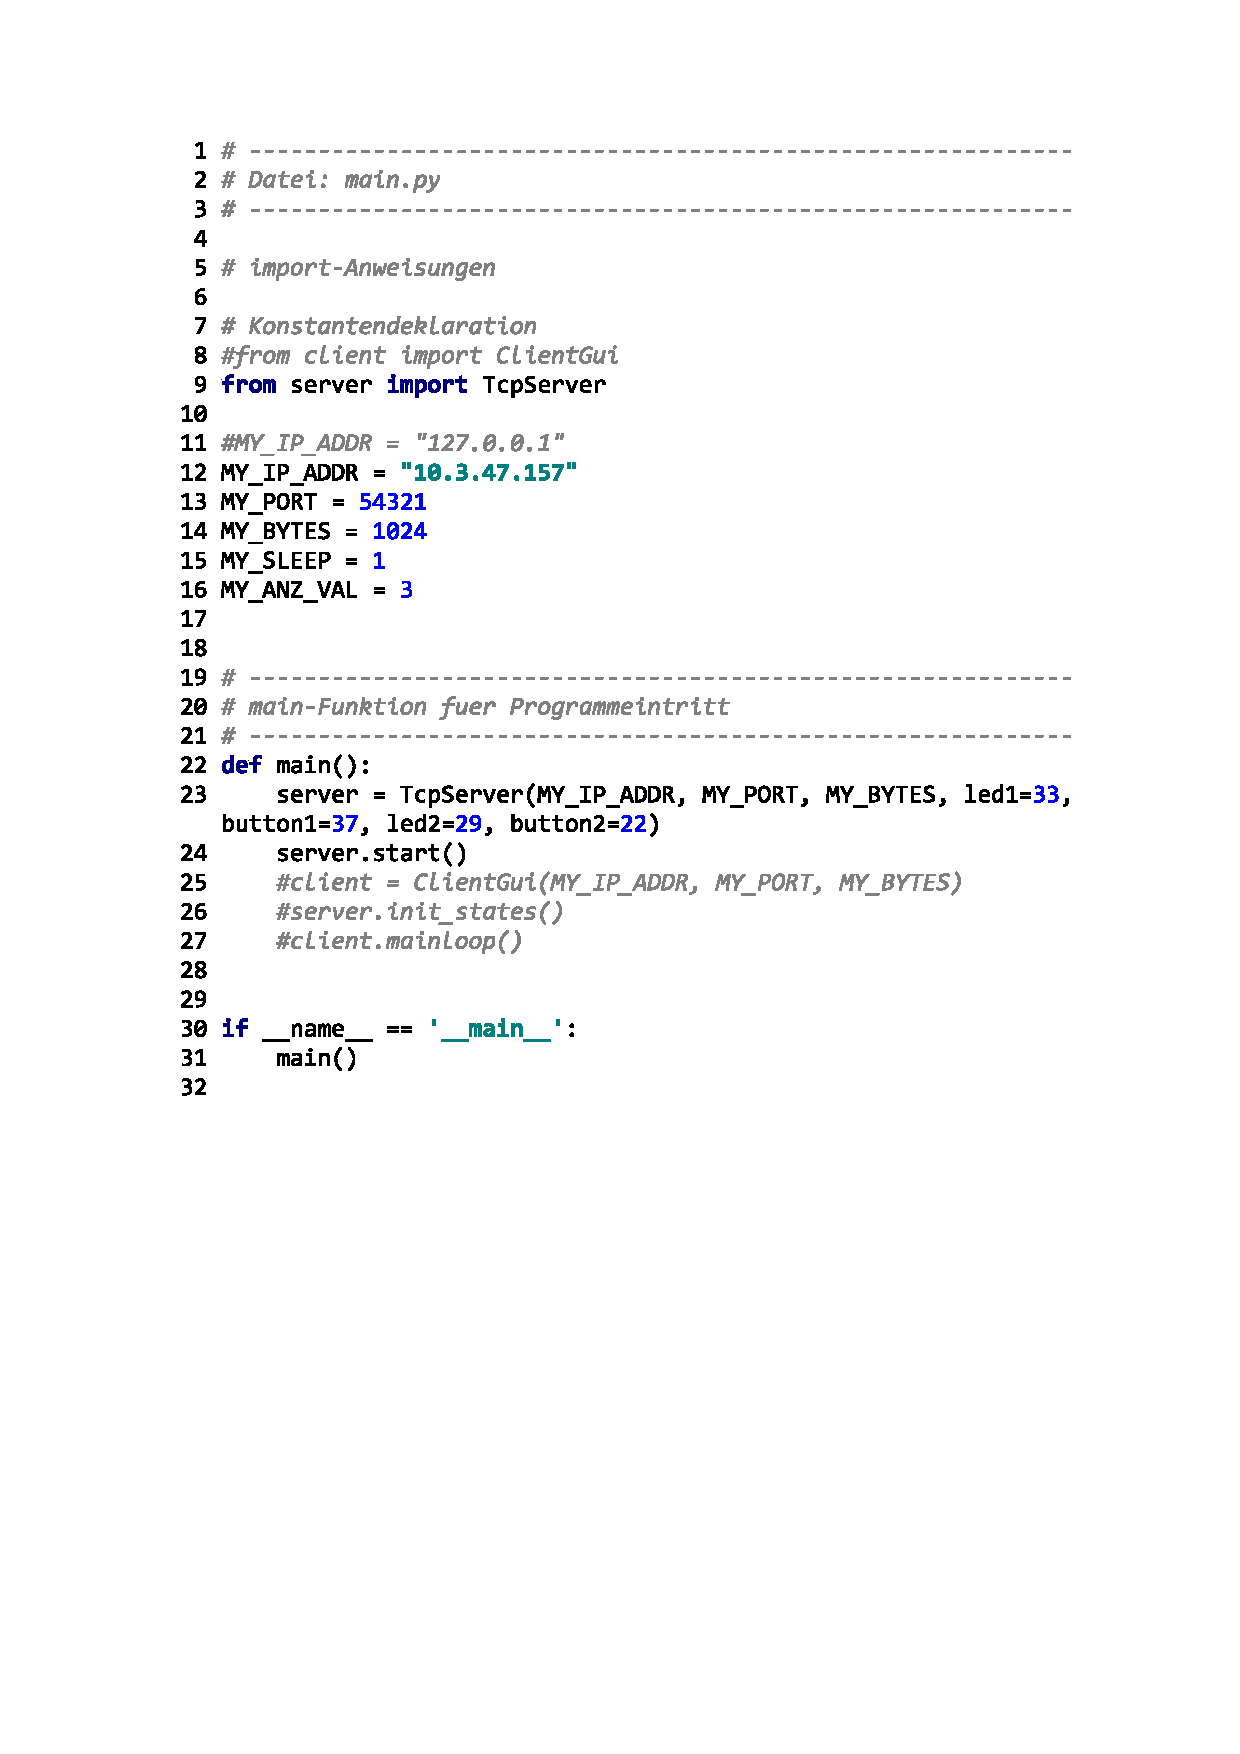
\includepdf[pages=1,scale=.8,fitpaper=true,pagecommand=\section{main\_server.py}]{main_server.pdf}
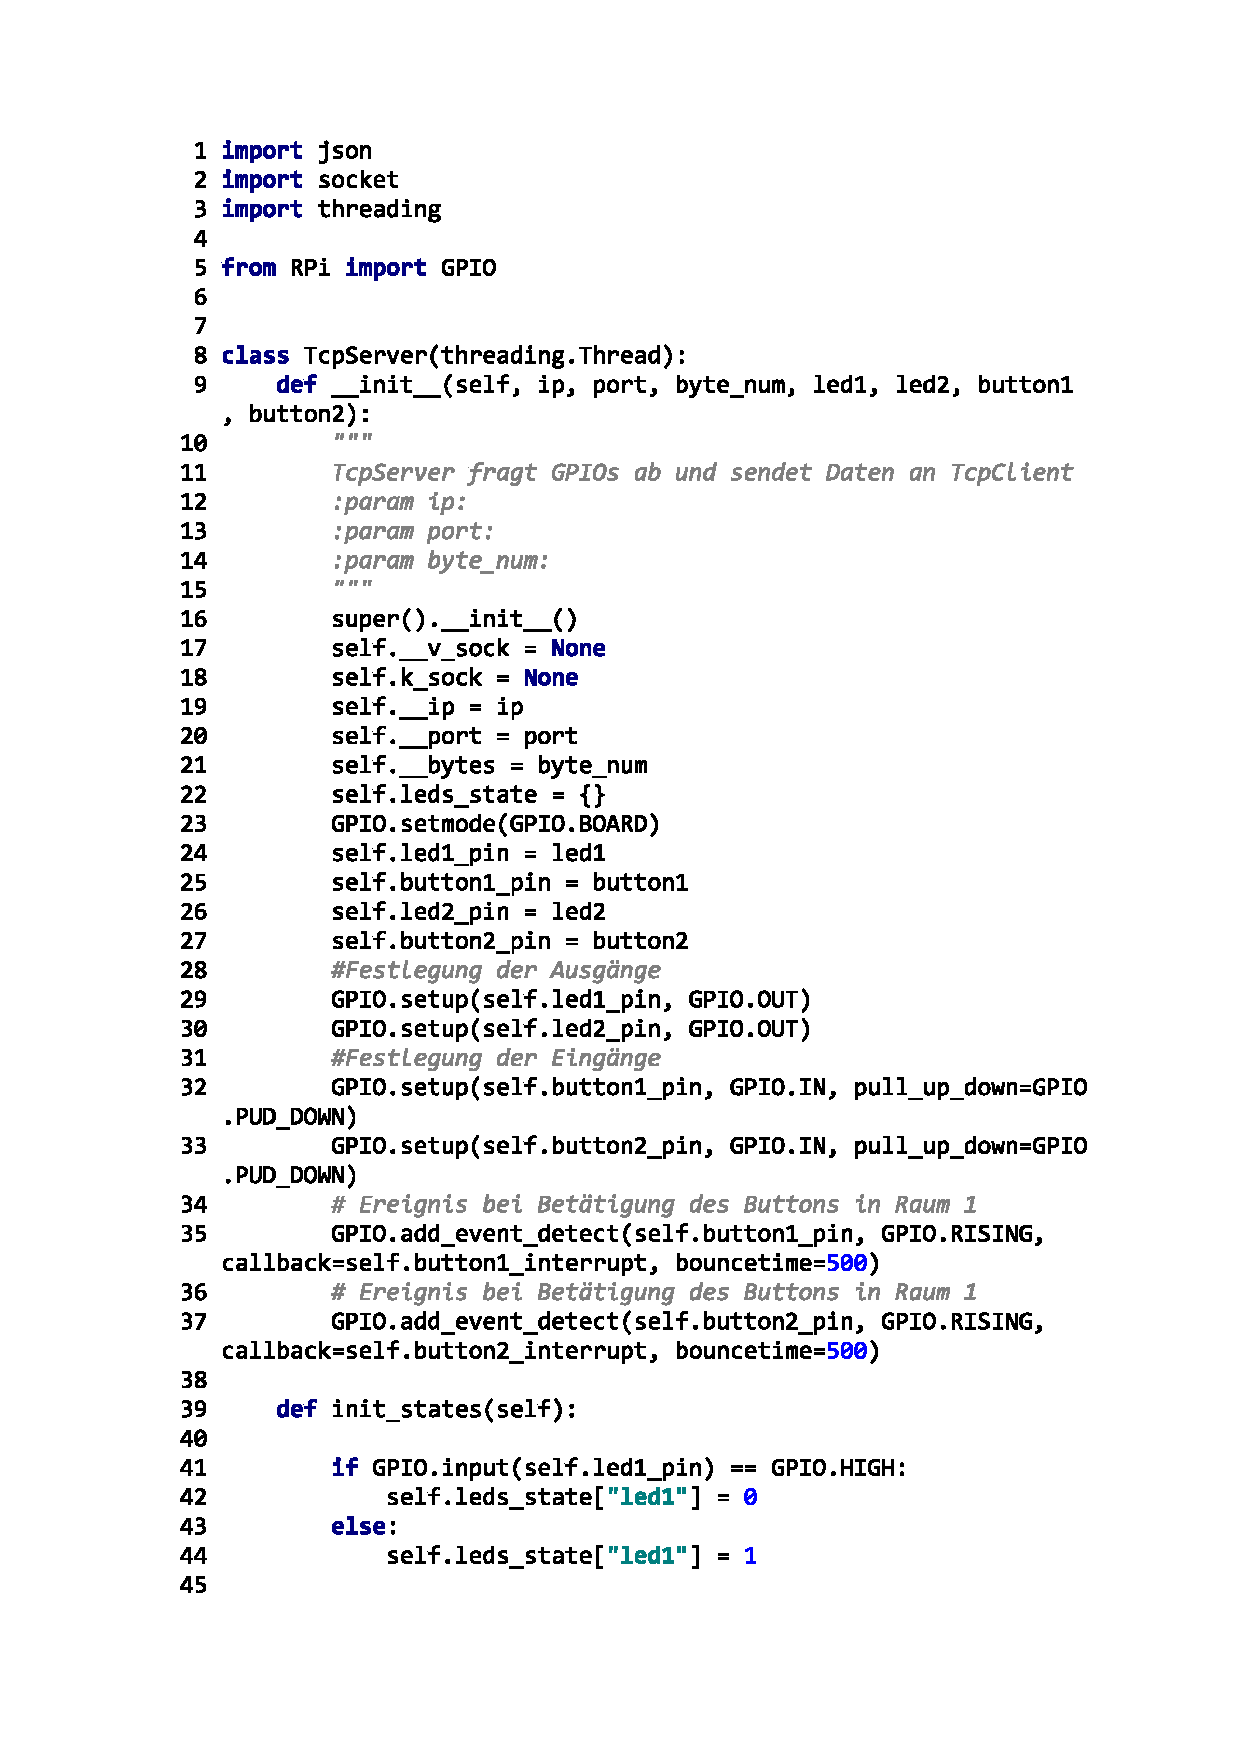
\includepdf[pages=1,scale=.8,fitpaper=true,pagecommand=\section{server.py}]{server.pdf}
\includepdf[pages=2-,scale=.8,pagecommand=\section*{}]{server.pdf}


%**********************************************************************************
%\chapter{Anhang: Quelltext des Clients} 

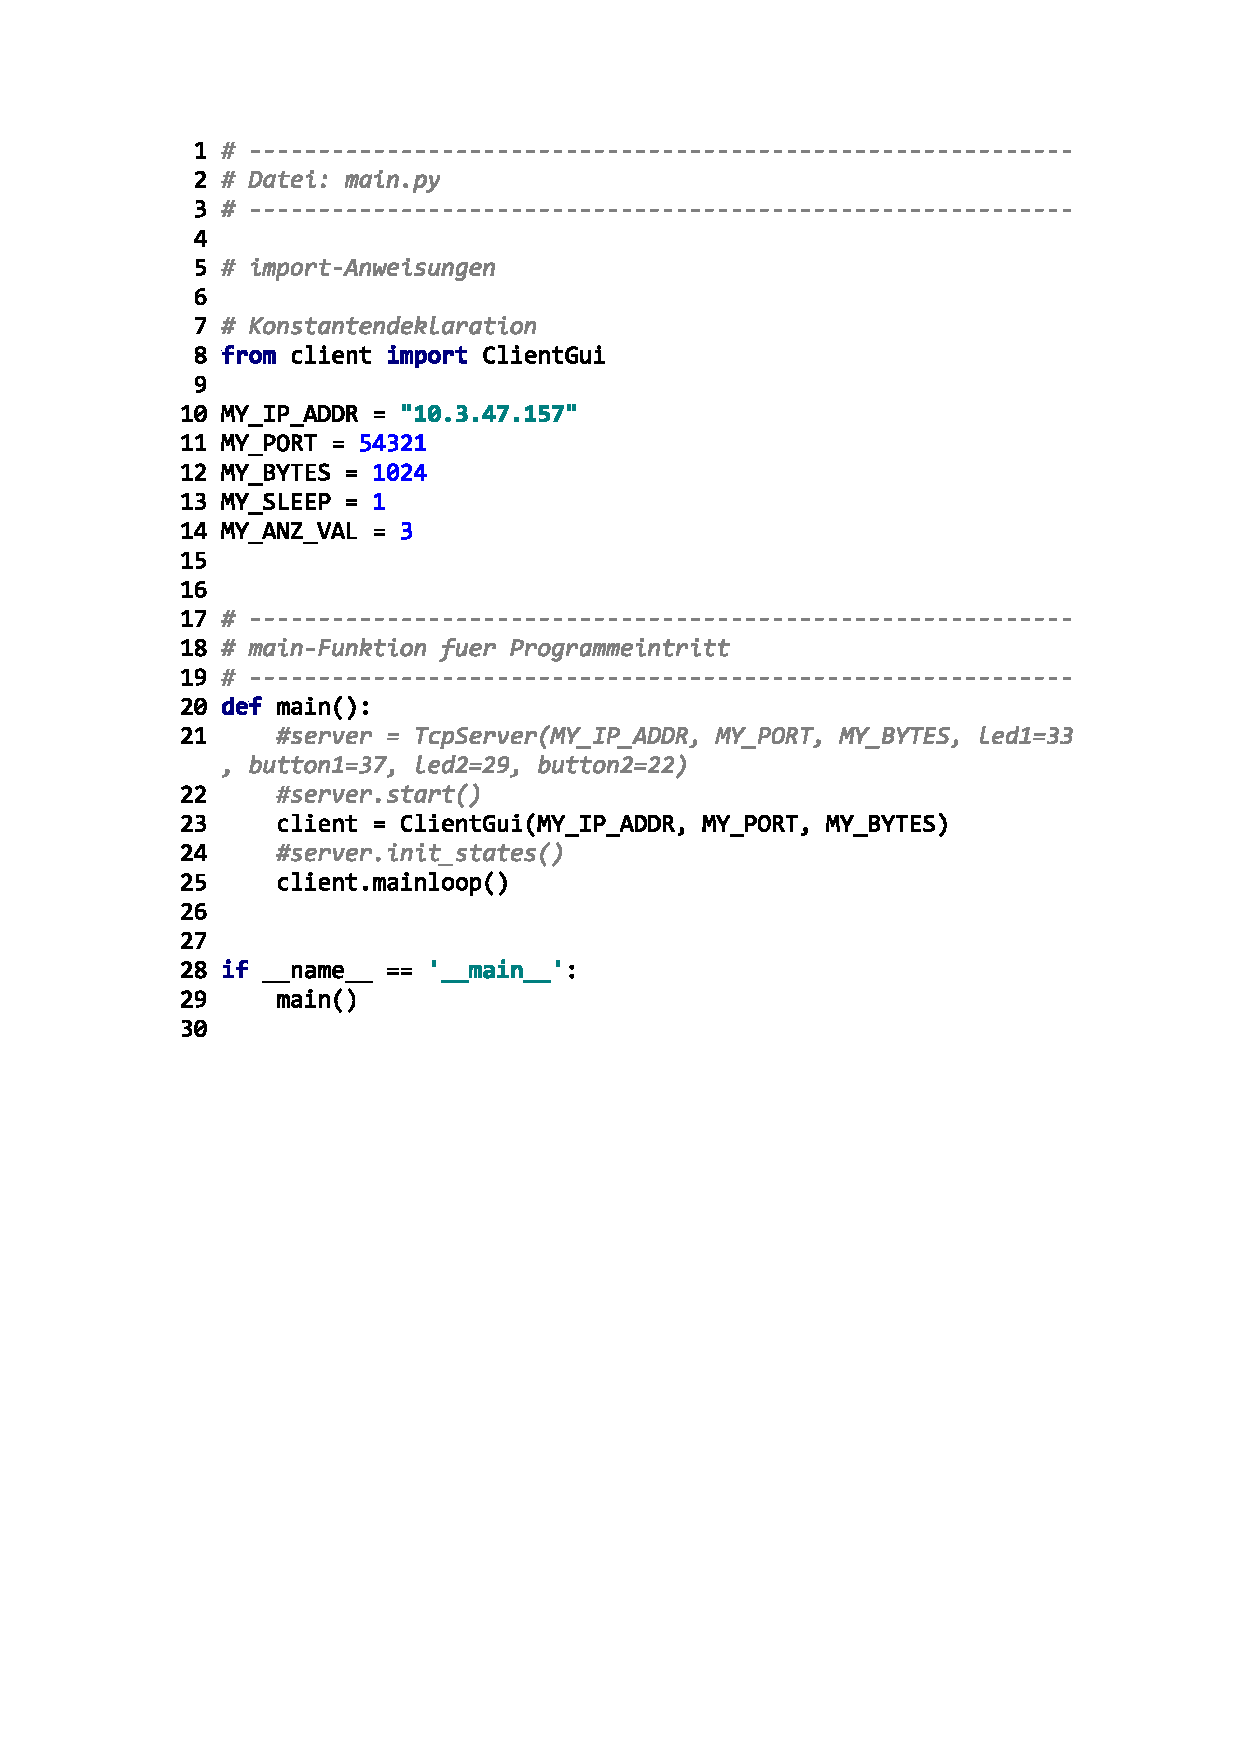
\includepdf[pages=1,scale=.8,fitpaper=true,pagecommand=\section{main\_client.py}]{main_client.pdf}
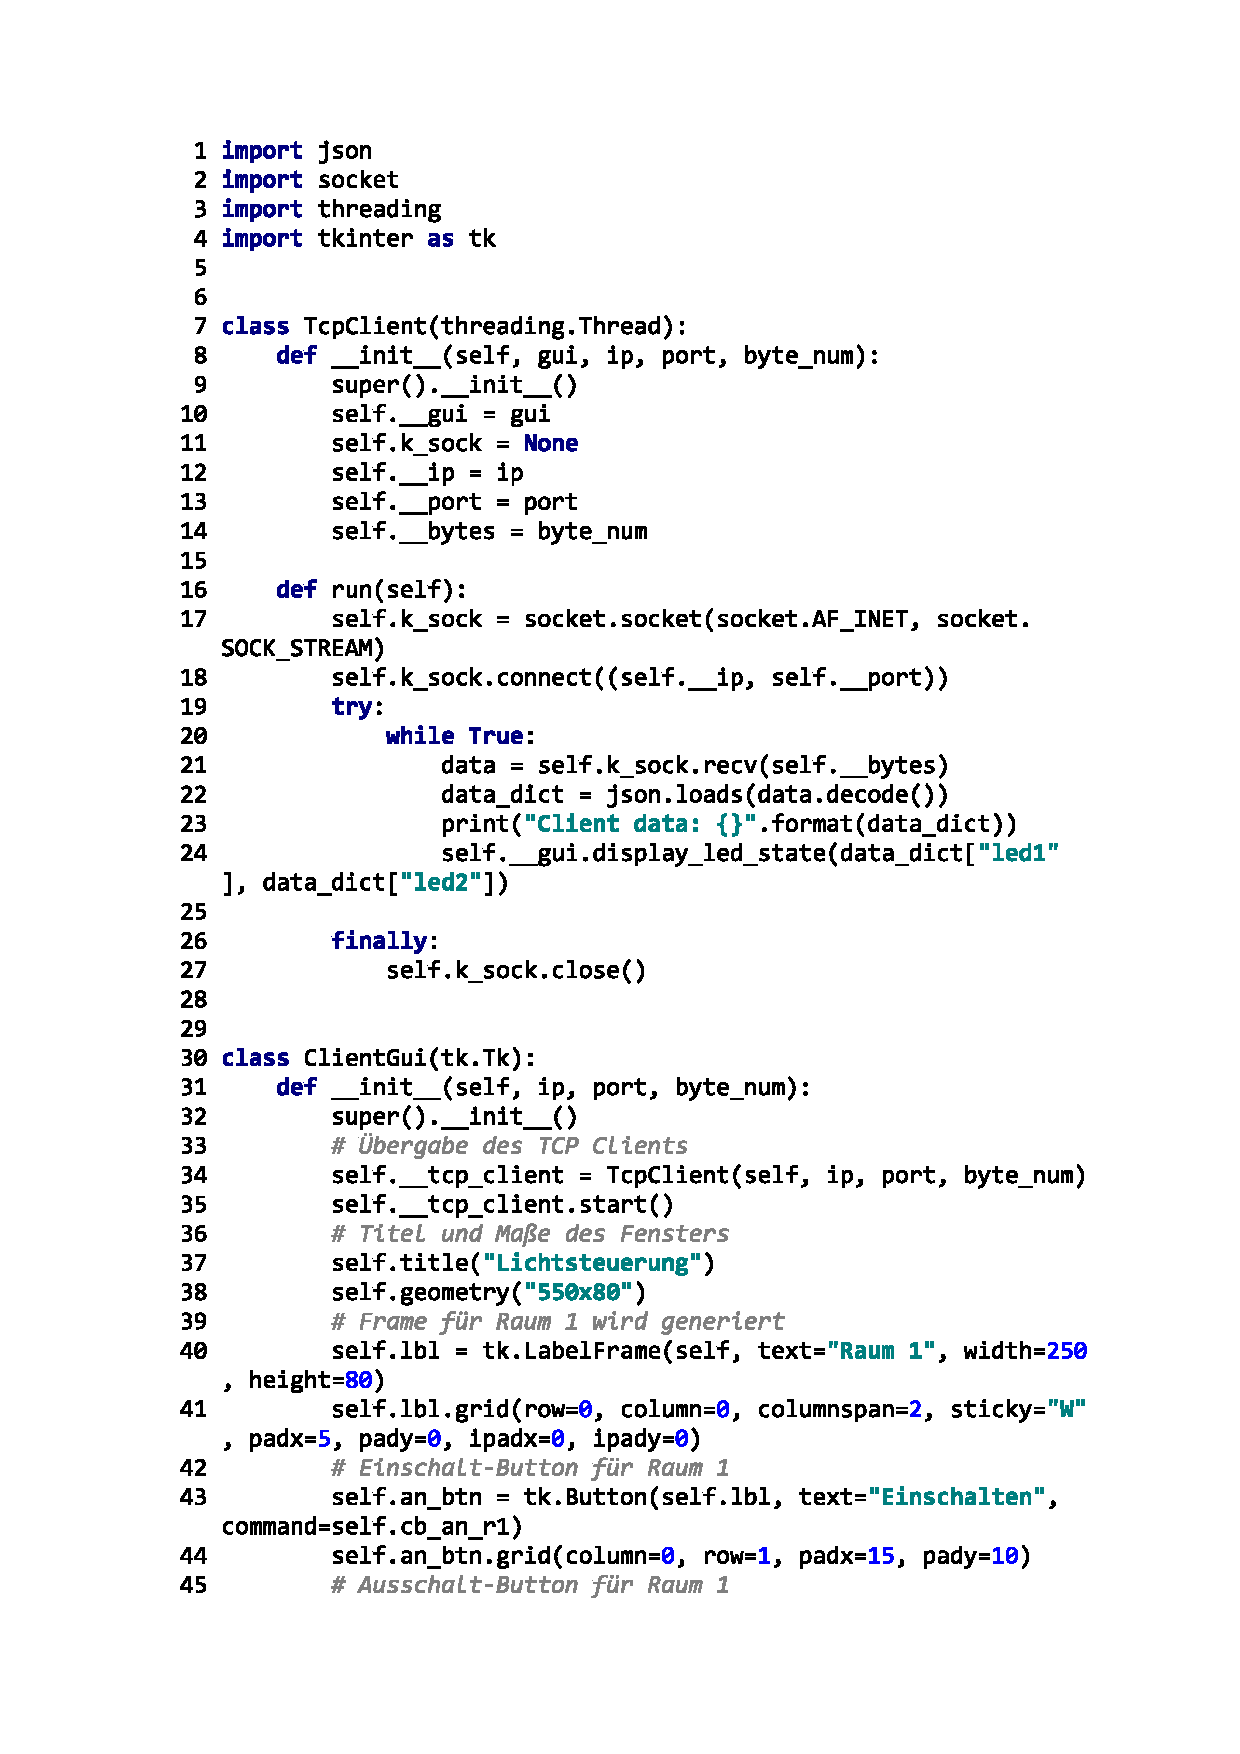
\includepdf[pages=1,scale=.8,fitpaper=true,pagecommand=\section{client.py}]{client.pdf}
\includepdf[pages=2-,scale=.8,pagecommand=\section*{}]{client.pdf}

\end{document}